\chapter{Evaluation and Analysis}

In the previous chapter, a few approaches that could improve the genetic solver were presented.
The best results give a combination of the genetic solver with added probabilities and parameter tuning.
Other methods like an adaptive crossover rate or population without duplicated individuals give less effect on the results.

On the other hand, we get valid results only for one problem. What if the problem will be smaller or bigger?
The evaluation was done to find out how all approaches work with different problem sizes. 

\section{Evaluation}

To evaluate genetic solver, a benchmark set of 36 problems was used.
Each problem with different parameters that describes them.
All parameters are:

\begin{itemize}
	\item variant - [2, 4] ,
	\item request - [1, 2, 4],
	\item depth - [2, 3, 4],
	\item resources - [50, 100].
\end{itemize}

This set was tested with several versions of the genetic solver:

\begin{itemize}
	\item basic (B),
	\item basic with tuned parameters (B-T),
	\item without hard-coded parameters and tuning (WHC-T) 
	\item with added parameters (NP),
	\item with added parameters and tuning (NP-T),
	\item with internally changeable crossover rate (ICCR),
	\item with internally changeable crossover rate and tuning (ICCR-T),
	\item without duplicates in the population (WD),
	\item without duplicates in the population and tuning (WD-T).
\end{itemize}

Each version of the genetic solver tries five times to solve each problem.

The benchmark set was run on an Intel Core i7-8700 CPU machine with 64Gb of memory using Fedora Server 29 and OpenJDK 1.8.0 201-b09.

Benchmark trying so solve each task, if a solution was valid, genetic solver start to solve next problem. If after five attempts the genetic solver did not find a valid solution, it proceeded to the next problem.

\begin{figure}
	\centering
	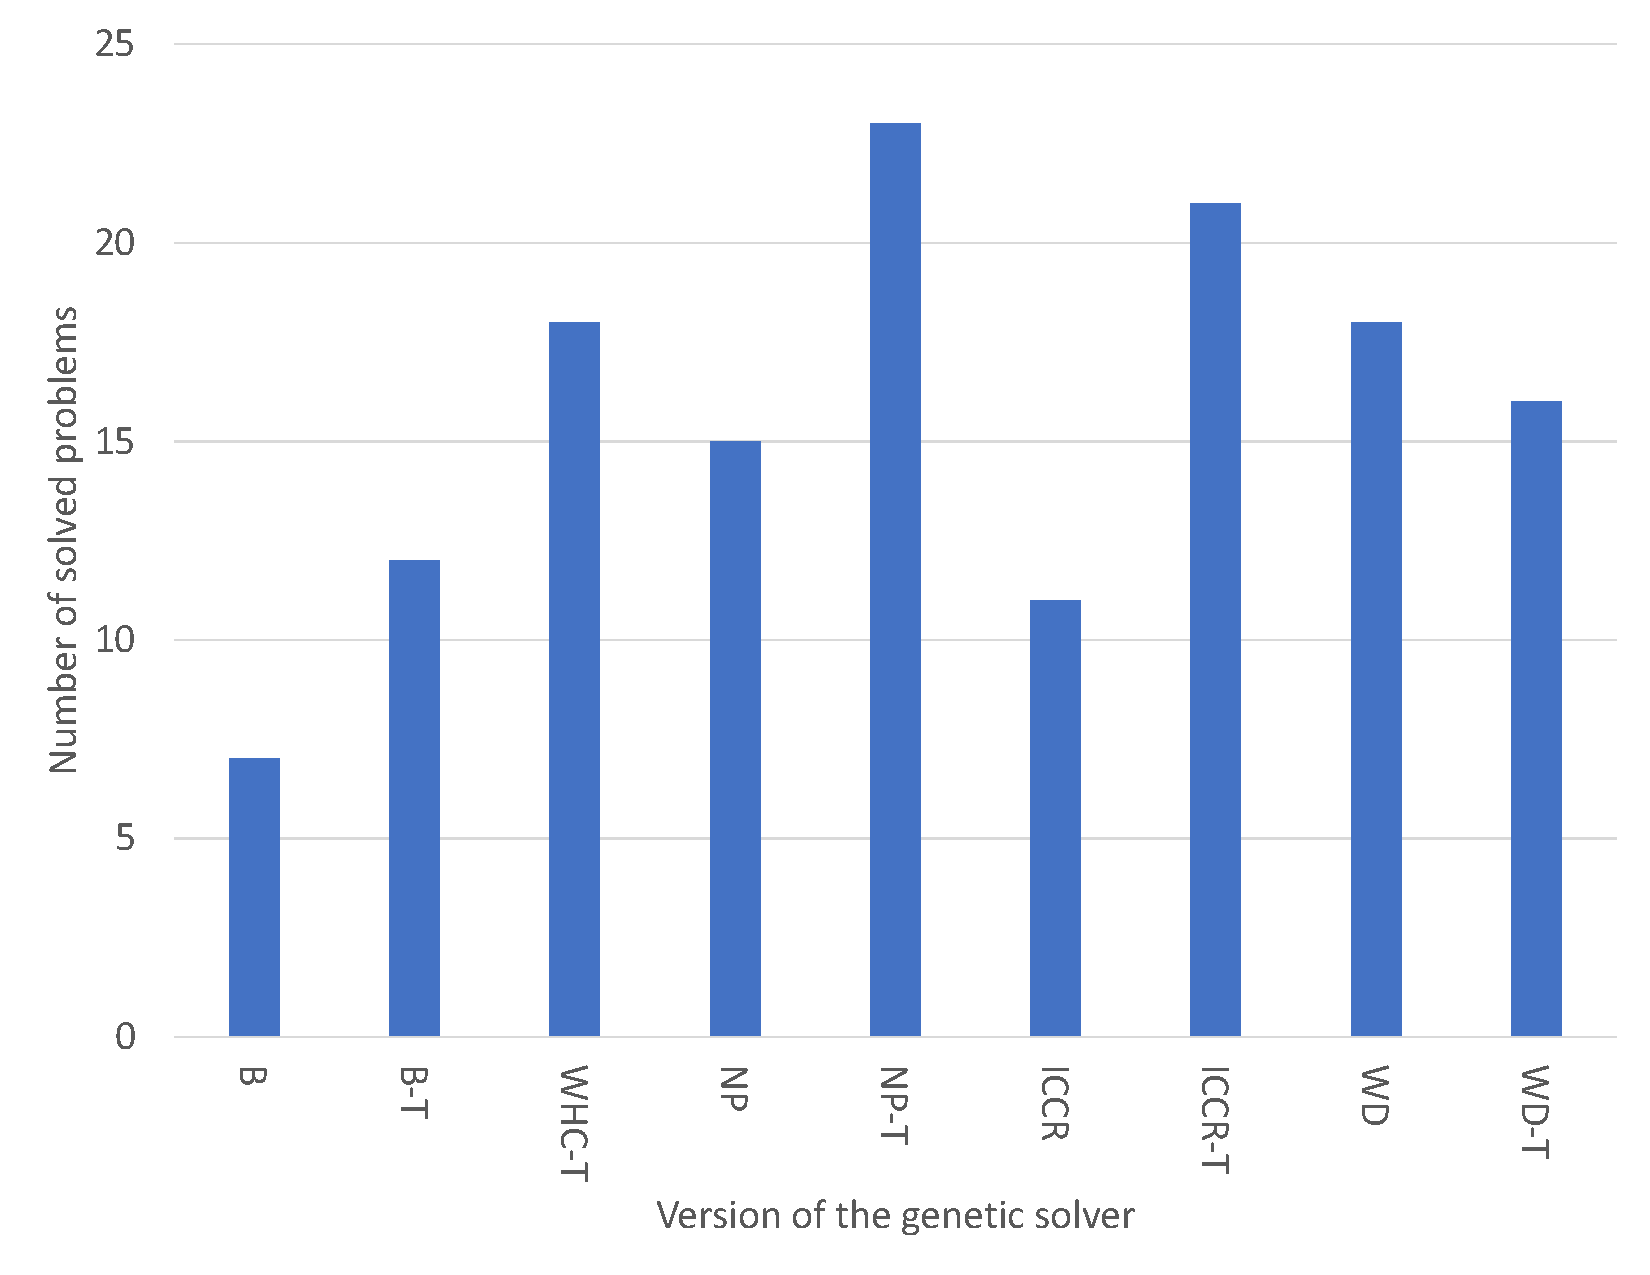
\includegraphics[width=\textwidth]{images/EvaluationNumberOfSolvedProblems.pdf}
	\caption[Number of problems for each version of the genetic solver]{Number of solved problems for each version of the genetic solver}
	\label{fig:EvaluationNumberOfSolvedProblems}
\end{figure}

Figure~\ref{fig:EvaluationNumberOfSolvedProblems} results of the benchmark. For each version of the genetic solver, a vertical bar was built. The height of the bar shows the number of solved problems from the benchmark set. The B version solved the least of problems than any other version. Almost in all cases, parameter tuning increases the number of solved problems. It also confirms the answer to \textbf{RQ1}. The comparison of N-T, WHC-T, and NP versions shows that the NP bar is higher than N-T but lower than WHC-T. This comparison confirms the first conclusion from Section~\ref{sec:NP}, that well-designed parameters are important for any algorithm. The combination of parameter engineering and parameter tuning in NP-T gives the best results. The same situation was for one problem in the previous chapter~(Figure~\ref{fig:boxplotsolverNoDuplicates}). The WD-T gives worse results than the untuned version. The possible reasons for such results were discussed in Section~\ref{sec:WD}. The result of the benchmark for the ICCR-T version contradicts the results obtained in the last section because the parameter tuning of the ICCR version gives the biggest improvement. In general, benchmark results for a set of 36 MQuAT problems correspond to the results for one problem.

The benchmark also shows that no one version of the genetic solver solved all problems from the set. Table~\ref{tab:ProblemsColorCoding} shows the results of the benchmark in the context of a solved or unsolved problem. Each row describes the result for a specified problem. The problem numbers contain in column \textit{Problem Id}. Black filled cell means that solver solved the problem. Table~\ref{tab:ProblemsColorCoding} also shows ids of problems that unsolved by all versions of the genetic solver.

\begin{table}
	\centering
	\caption{Problem color coding}\label{tab:ProblemsColorCoding}
	\resizebox*{\textwidth}{\textheight}{
		\begin{tabular}{c | c | c | c | c | c | c | c | c | c}
			\hline
			\rotatebox{90}{Problem Id} & \rotatebox{90}{B} & \rotatebox{90}{B-T} & \rotatebox{90}{WHC-T} & \rotatebox{90}{NP} & \rotatebox{90}{NP-T} & \rotatebox{90}{ICCR} & \rotatebox{90}{ICCR-T} & \rotatebox{90}{WD} & \rotatebox{90}{WD-T} \\
			\hline			
			1 & \cellcolor{black} & \cellcolor{black} & \cellcolor{black} & \cellcolor{black} & \cellcolor{black} & \cellcolor{black} & \cellcolor{black} & \cellcolor{black} & \cellcolor{black} \\ 
			2 &   &   & \cellcolor{black} &   & \cellcolor{black} &   &   & \cellcolor{black} & \cellcolor{black}  \\
			3 &   &   &   &   & \cellcolor{black} &   &   & \cellcolor{black} &  \\
			4 &   & \cellcolor{black} & \cellcolor{black} & \cellcolor{black} & \cellcolor{black} & \cellcolor{black} & \cellcolor{black} & \cellcolor{black} & \cellcolor{black} \\
			5 &   &   &   &   & \cellcolor{black} &   & \cellcolor{black} &   & \\
			6 &   &   &   &   &   &   &   &   & \\
			7 &   & \cellcolor{black} & \cellcolor{black} & \cellcolor{black} & \cellcolor{black} &   & \cellcolor{black} & \cellcolor{black} & \cellcolor{black}\\
			8 &   &   &   &   &   &   &   &   & \\
			9 &   &   &   &   &   &   &   &   & \\
			10 & \cellcolor{black} & \cellcolor{black} & \cellcolor{black} & \cellcolor{black} & \cellcolor{black} & \cellcolor{black} & \cellcolor{black} & \cellcolor{black} & \cellcolor{black} \\
			11 &   &   & \cellcolor{black} & \cellcolor{black} & \cellcolor{black} & \cellcolor{black} & \cellcolor{black} & \cellcolor{black} & \cellcolor{black} \\
			12 &   &   &   &   & \cellcolor{black} &   & \cellcolor{black} & \cellcolor{black} &   \\
			13 & \cellcolor{black} & \cellcolor{black} & \cellcolor{black} & \cellcolor{black} & \cellcolor{black} & \cellcolor{black} & \cellcolor{black} & \cellcolor{black} & \cellcolor{black} \\
			14 &   &   &   &   & \cellcolor{black} &   & \cellcolor{black} &   &   \\
			15 &   &   &   &   &   &   &   &   & \\
			16 &   & \cellcolor{black} & \cellcolor{black} & \cellcolor{black} & \cellcolor{black} &   & \cellcolor{black} &   & \cellcolor{black} \\
			17 &   &   &   &   &   &   &   &   & \\
			18 &   &   &   &   &   &   &   &   & \\
			19 & \cellcolor{black} & \cellcolor{black} & \cellcolor{black} & \cellcolor{black} & \cellcolor{black} & \cellcolor{black} & \cellcolor{black} & \cellcolor{black} & \cellcolor{black}\\
			20 &   &   & \cellcolor{black} & \cellcolor{black} & \cellcolor{black} & \cellcolor{black} & \cellcolor{black} & \cellcolor{black} & \cellcolor{black} \\
			21 &   &   &   &   & \cellcolor{black} &   & \cellcolor{black} &   & \\
			22 & \cellcolor{black} & \cellcolor{black} & \cellcolor{black} &   & \cellcolor{black} & \cellcolor{black} & \cellcolor{black} & \cellcolor{black} & \cellcolor{black} \\
			23 &   &   & \cellcolor{black} & \cellcolor{black} & \cellcolor{black} &   & \cellcolor{black} & \cellcolor{black} &  \\
			24 &   &   &   &   &   &   &   &   & \\
			25 &   &   & \cellcolor{black} & \cellcolor{black} & \cellcolor{black} &   & \cellcolor{black} &   & \cellcolor{black} \\
			26 &   &   &   &   &   &   &   &   & \\
			27 &   &   &   &   &   &   &   &   & \\
			28 & \cellcolor{black} & \cellcolor{black} & \cellcolor{black} & \cellcolor{black} & \cellcolor{black} & \cellcolor{black} & \cellcolor{black} & \cellcolor{black} & \cellcolor{black} \\
			29 &   & \cellcolor{black} & \cellcolor{black} & \cellcolor{black} & \cellcolor{black} & \cellcolor{black} & \cellcolor{black} & \cellcolor{black} & \cellcolor{black} \\
			30 &   &   &   &   &   &   &   &   & \\
			31 & \cellcolor{black} & \cellcolor{black} & \cellcolor{black} & \cellcolor{black} & \cellcolor{black} & \cellcolor{black} & \cellcolor{black} & \cellcolor{black} & \cellcolor{black} \\
			32 &   &   & \cellcolor{black} & \cellcolor{black} & \cellcolor{black} &   & \cellcolor{black} & \cellcolor{black} &  \\ 
			33 &   &   &   &   &   &   &   &   & \\
			34 &   & \cellcolor{black} & \cellcolor{black} &   & \cellcolor{black} &   & \cellcolor{black} & \cellcolor{black} & \cellcolor{black} \\
			35 &   &   &   &   &   &   &   &   & \\
			36 &   &   &   &   &   &   &   &   & \\
			\hline
		\end{tabular}
	}
\end{table}

Unsolved tasks are presented in Table~\ref{tab:UnsolvedProblems}. It shows parameters that specified the problem. We can see, there are a few types of unsolved problems are exist. All versions of the genetic solver could not solve the problem that contains two or more requests, and the depth is three or more. The exception for this definition is a problem number 30. It has one request and depth four, but it also has variants four and resources - 100 and genetic solvers could not solve it.


\begin{table}
	\centering
	\caption{Not solved problems}\label{tab:UnsolvedProblems}
	\resizebox{\textwidth}{!}{
		\begin{tabular}{c c c c c}
			\hline
			Problem Id & variants & requests & depth & resources \\
			\hline			
			6 & 2 & 2 & 4 & 50 \\
			8 & 2 & 4 & 3 & 50 \\
			9 & 2 & 4 & 4 & 50 \\
			15 & 2 & 2 & 4 & 100 \\
			17 & 2 & 4 & 3 & 100 \\
			18 & 2 & 4 & 4 & 100 \\
			24 & 4 & 2 & 4 & 50 \\
			26 & 4 & 4 & 3 & 50 \\
			27 & 4 & 4 & 4 & 50 \\
			30 & 4 & 1 & 4 & 100 \\
			33 & 4 & 2 & 4 & 100 \\
			35 & 4 & 4 & 3 & 100 \\
			36 & 4 & 4 & 4 & 100 \\
			\hline
		\end{tabular}
	}
\end{table}

If a genetic solver could solve some problems, then solutions have a quality.
Let us now discuss the quality of the received results. Figure~\ref{fig:EnergyPercentage} shows the percentage of the deviation from the optimum for problems that solved by all versions of the genetic solver. The optimum values for problems received by the ILP solver. If the percentage of the deviation is zero, that means that the received solution is \textbf{optimal}. The max deviation is near 30\% for the B version with problem 31. However, other versions give solutions with deviation from optimal that less than 10\% or even optimal solutions for the NP-T version. There are high deviations from optimum in problems number 13 for tuned versions of the genetic solver such as B-T, NP-T, ICCR-T, and WD-T. Nevertheless, WHC-T and untuned versions give a near-optimal solution with minimal deviation. The ICCR version gives a much higher percentage of deviation than other versions in problem 19.

\begin{figure}
	\centering
	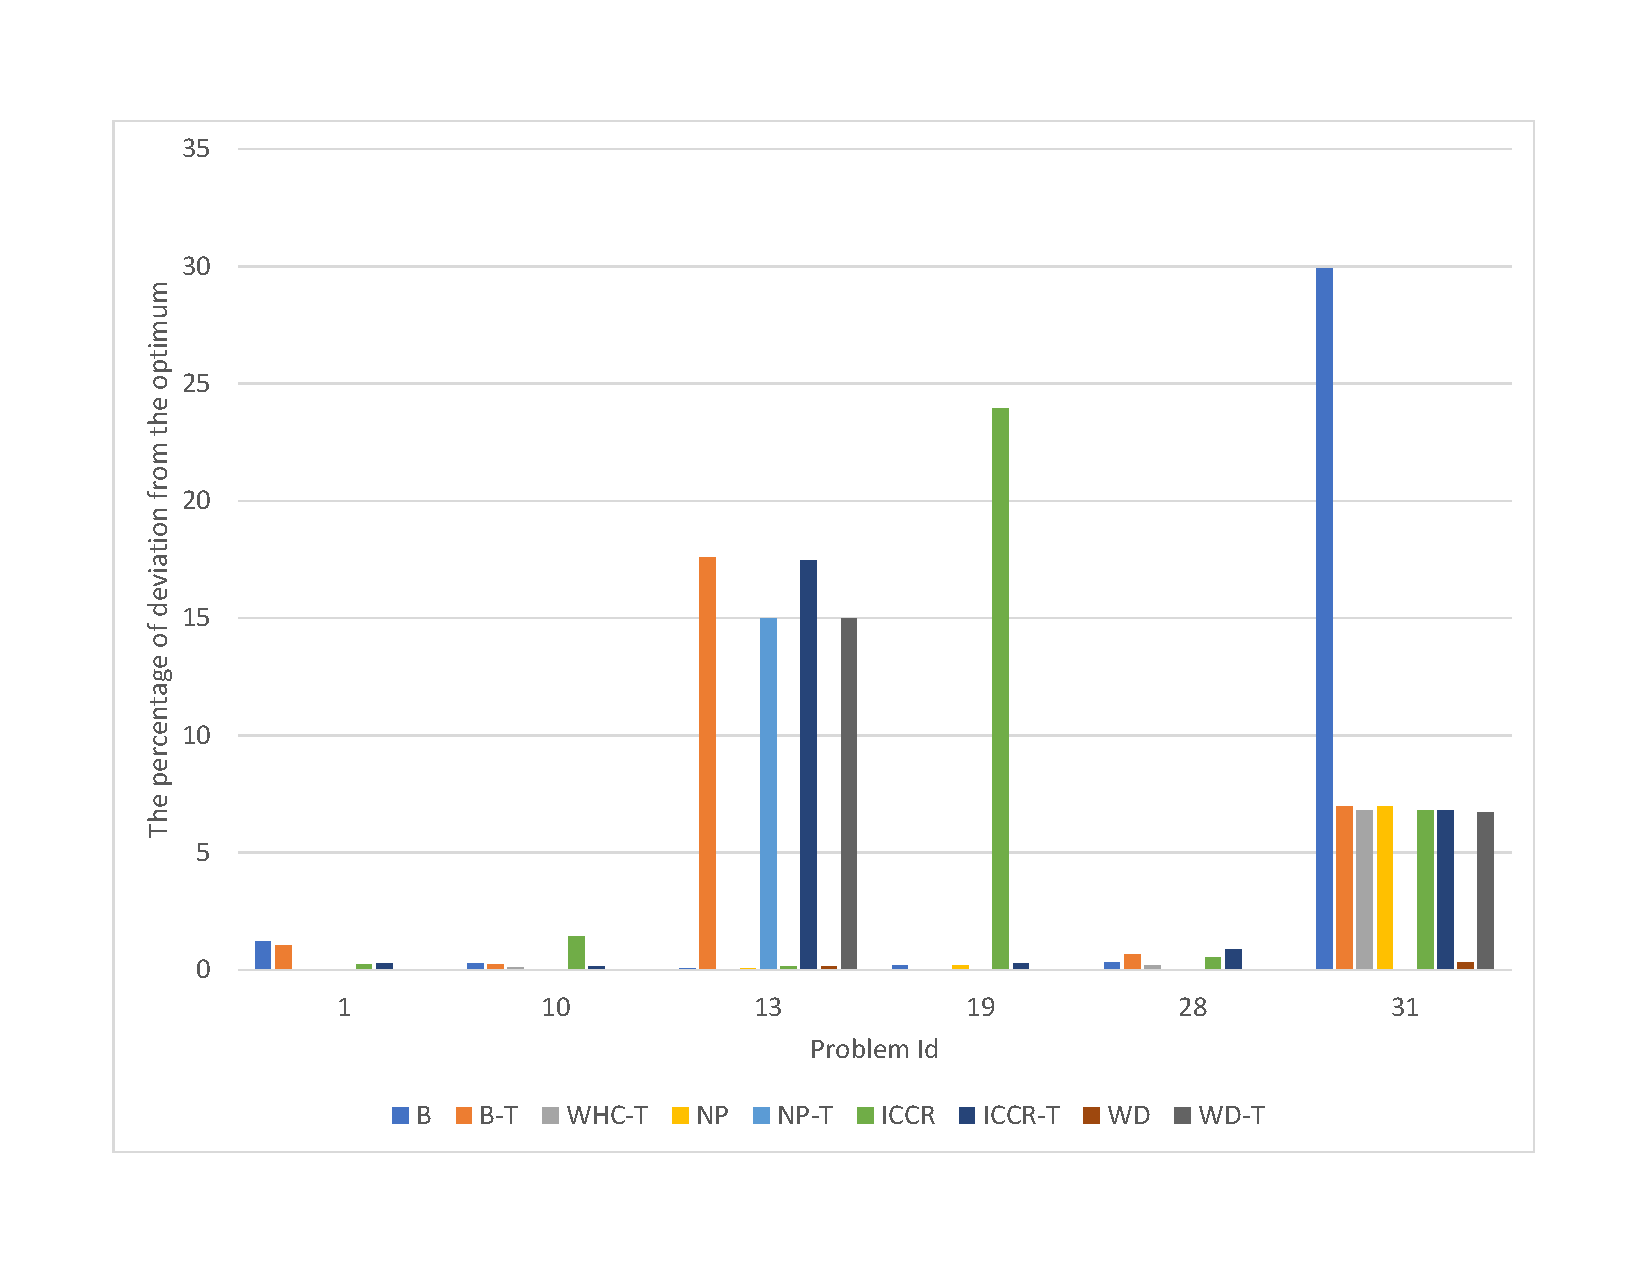
\includegraphics[width=\textwidth]{images/EnergyPercentage.pdf}
	\caption[]{}
	\label{fig:EnergyPercentage}
\end{figure}

Figure~\ref{fig:EnergyPercentage} also shows that the deviation is increasing for big size problems. To confirm that fact, we take two problems with different sizes~(Figures~\ref{fig:SmallMediumProblemEnergy}). These problems solved by all version of the genetic solver except the B version. Figure~\ref{fig:SmallProblemEnergy} shows the percentage of deviation from optimum for a small size problem. This problem's parameters are:
\begin{itemize}
	\item variants: 2,
	\item requests: 2,
	\item depth: 2,
	\item resources: 50.
\end{itemize}.

The quality of results for the problem is near-optimal, because the deviation is less than one percent. The NP-T and WD-T versions give an optimal solution for the problem.

On the side, Figure~\ref{fig:MediumProblemEnergy} shows the percentage of deviation from optimum for a bigger size problem. This problem's parameters are:
\begin{itemize}
	\item variants: 4,
	\item requests: 1,
	\item depth: 3,
	\item resources: 100.
\end{itemize}.

The quality of results in a case of the bigger problem is much worse. The minimal deviation is 35\% for the NP-T version because the deviation is less than one percent. The NP-T and WD-T versions give an optimal solution for the problem. The WD and WD-T versions give less valid solutions in the benchmark, but the quality of the solution is higher. The quality of the solution from other solvers is lower because the percentage of the deviation is more than 100\%. The reason why the quality of solutions is decreasing with a bigger size of the problem could be a higher number of hardware resources. The higher number of resources means that more hardware resources could satisfy the requirements of the software component. The genetic solver could not find best-suited resources for requested components, and as a result, quality is decreasing. 


\begin{figure}
	\centering
	\begin{subfigure}{0.45\textwidth}
		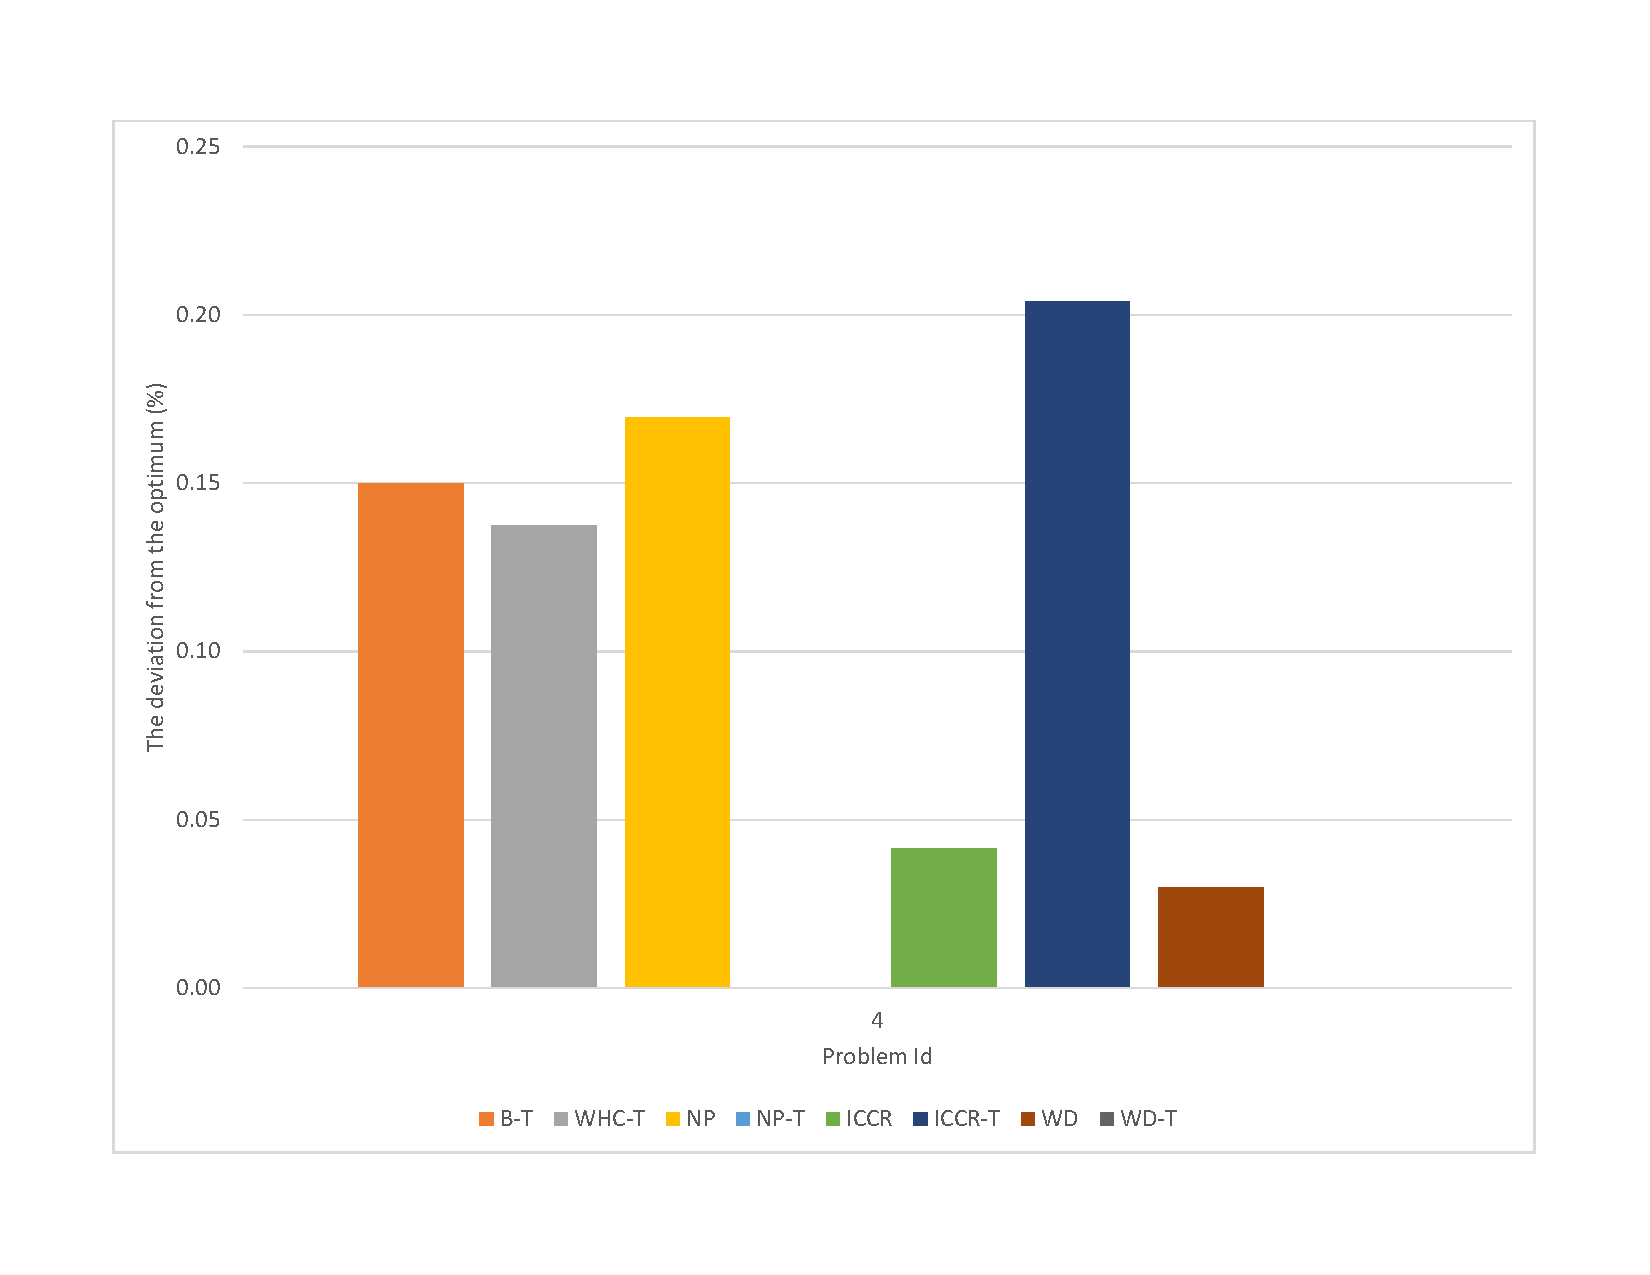
\includegraphics[width=\textwidth]{images/EnergyDeviationSmallProblem.pdf}
		\caption{$y=x$}
		\label{fig:SmallProblemEnergy}
	\end{subfigure}
	\hfill
	\begin{subfigure}{0.45\textwidth}
		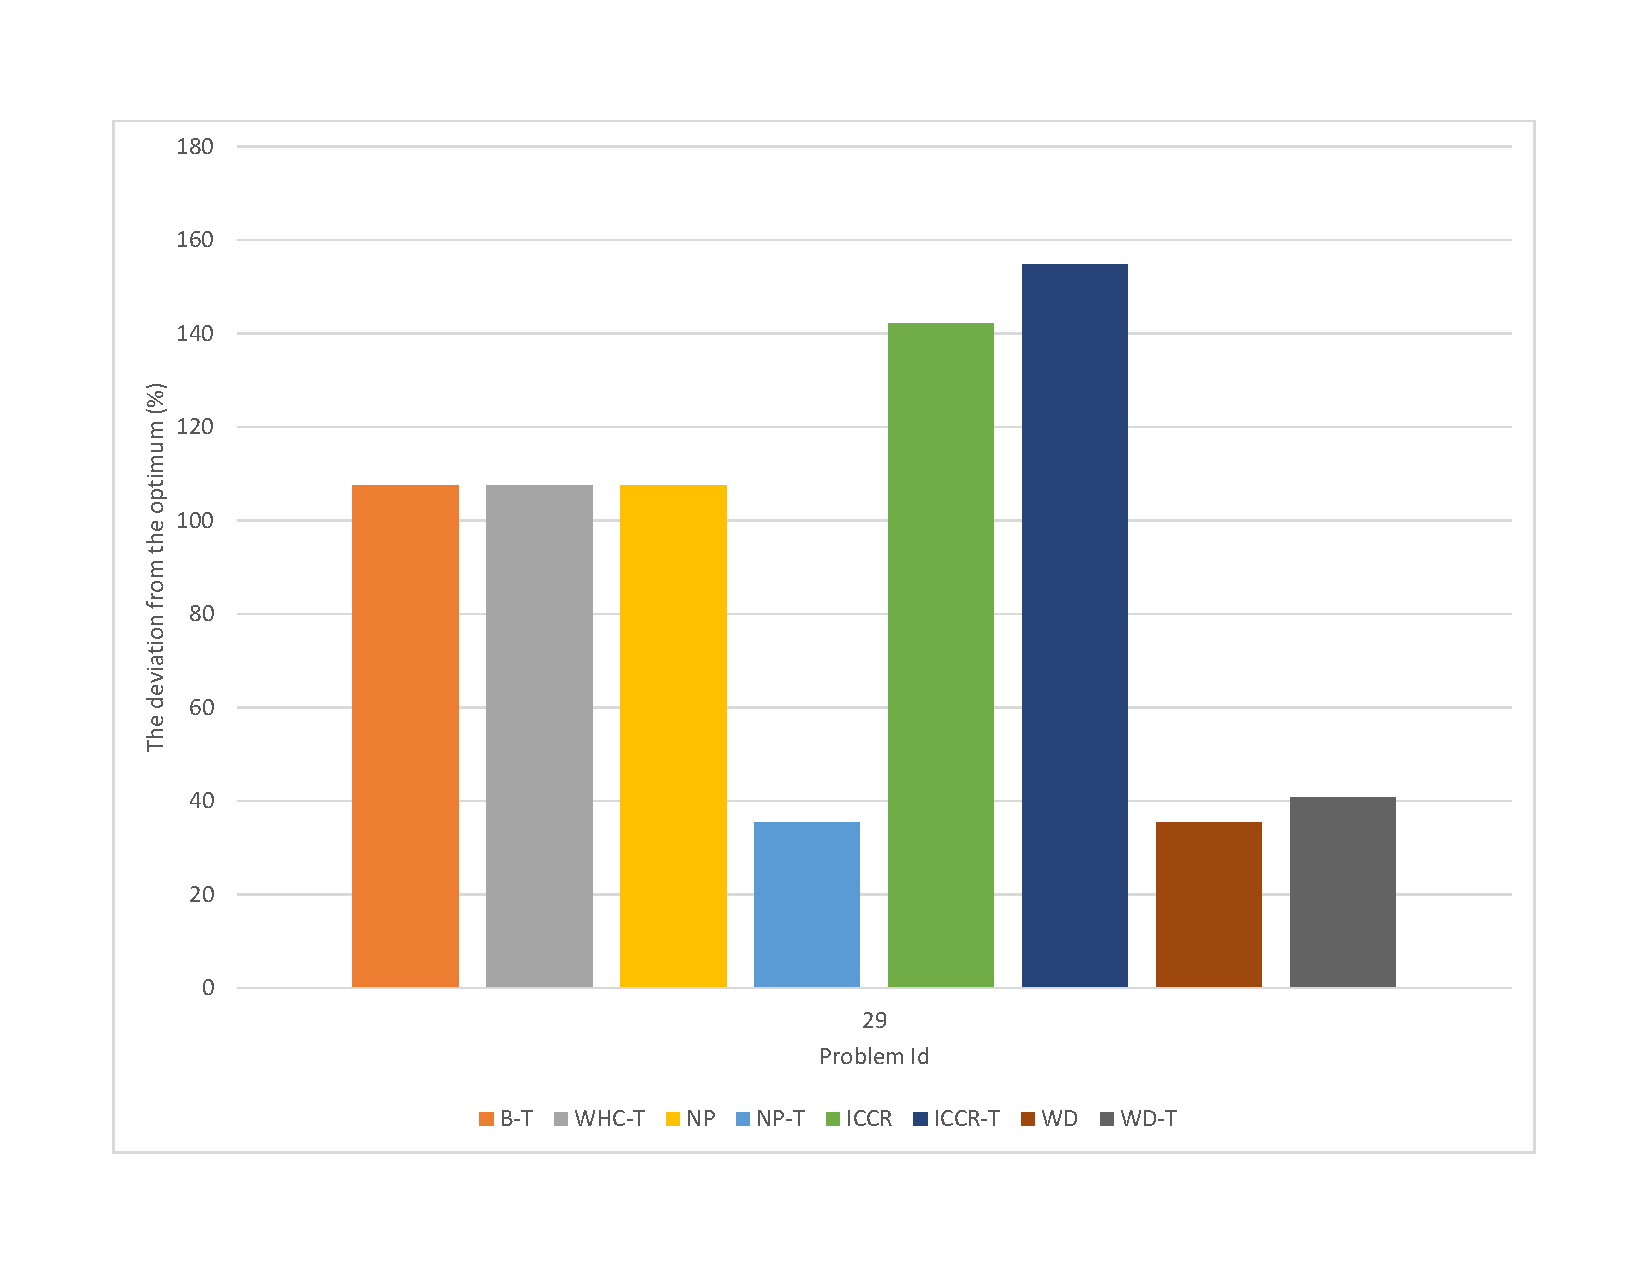
\includegraphics[width=\textwidth]{images/EnergyDeviationMediumProblem.pdf}
		\caption{$y=x$}
		\label{fig:MediumProblemEnergy}
	\end{subfigure}	
	\caption{Three simple graphs}
	\label{fig:SmallMediumProblemEnergy}	
\end{figure}


This section shows that modification that we made improve the results of the genetic solver. The NP-T version solved three times more problems than the B version. We evaluated the quality of solutions. As a result of the quality evaluation, we make two conclusions. First, modified versions of the genetic solver also improve the quality of the results. Second, the quality is decreasing for a bigger size of the problem.
However, there are problems from the set that could not be solved by the genetic solver.


\section{Analysis}

Benchmark showed that a genetic solver could not solve all MQuAT problems from the evaluation set.
In this section, we presented an analysis of results, reasons why described in Chapter~\ref{chapter:Implementation} approaches, and optimizations have lower efficiency that we need.

Firstly, let us discuss the reasons why modifications that we made improve the genetic solver. After that we will concentrate on the reasons why not all tasks could be solved.

There is a few reasons why the genetic solver with our modifications could solve more problems than the B version. First of all, parameter tuning was performed for all versions. Optimized values of parameters gives a better results as it showed in the previous section. The second reason is a new probabilities that we added in Section~\ref{sec:NP}.These probabilities give a possibility to randomly change the position of the Crossover and mutation points and as a result, the genetic solver gives results that a bit worse than parameter tuning. 

Nevertheless, not all tasks were solved. The one of the reasons of such result is parameter tuning. We optimized parameters for specific problems, that we described at the beginning of Chapter~\ref{chapter:Implementation}.

There is a \textbf{"no free lunch" (NFL) theorem}\cite{wolpert1996, wolpert1997} that describes the obtained results. The NFL theorem says that if an algorithm works well with a certain class of tasks, then it must pay for it with a deterioration in performance on the set of all remaining problems.

Another reason could be many parameters of the genetic solver or their dependencies between themselves. As a result, the user and BRISE do not know details about the search space of parameters and could not find an optimized set. 

We start an analysis with search space representation. For this representation, we performed measurements for more than three thousand configurations using BRISE in the Search space exploration mode with NP version of the genetic solver. This mode was described in Section~\ref{sec:BRISE}. For this type of analysis we use the same problem as in Chapter~\ref{chapter:Implementation} and it has parameter values:
\begin{itemize}
	\item variants: 10,
	\item requests: 15,
	\item depth: 2,
	\item resources: 5,
	\item timeout: 5 minutes.
\end{itemize}

The search space representation as a parallel coordinates plot showed in Figure~\ref{fig:SearchSpaceViewFull}.
Each parameter is represented in the plot as a vertical line that contains all possible values of the parameter. Each configuration that was measured showed on the plot as a line that connects all values that describe itself. The last vertical line and the color shows the number of contract violations that gives the configuration. The more dark color means fewer contract violations and vise versa, the lighter color gives a higher number of contract violations.

\begin{figure}
	\centering
	\includegraphics[width=\textwidth]{images/SPEA2.pdf}
	\caption[]]{}
	\label{fig:SearchSpaceViewFull}
\end{figure}

Figure~\ref{fig:SearchSpaceViewFull} shows that search space of parameters contains configuration that led to results with different number of contract violations. There is no any visible dependencies between parameters. 

\begin{figure}
	\centering
	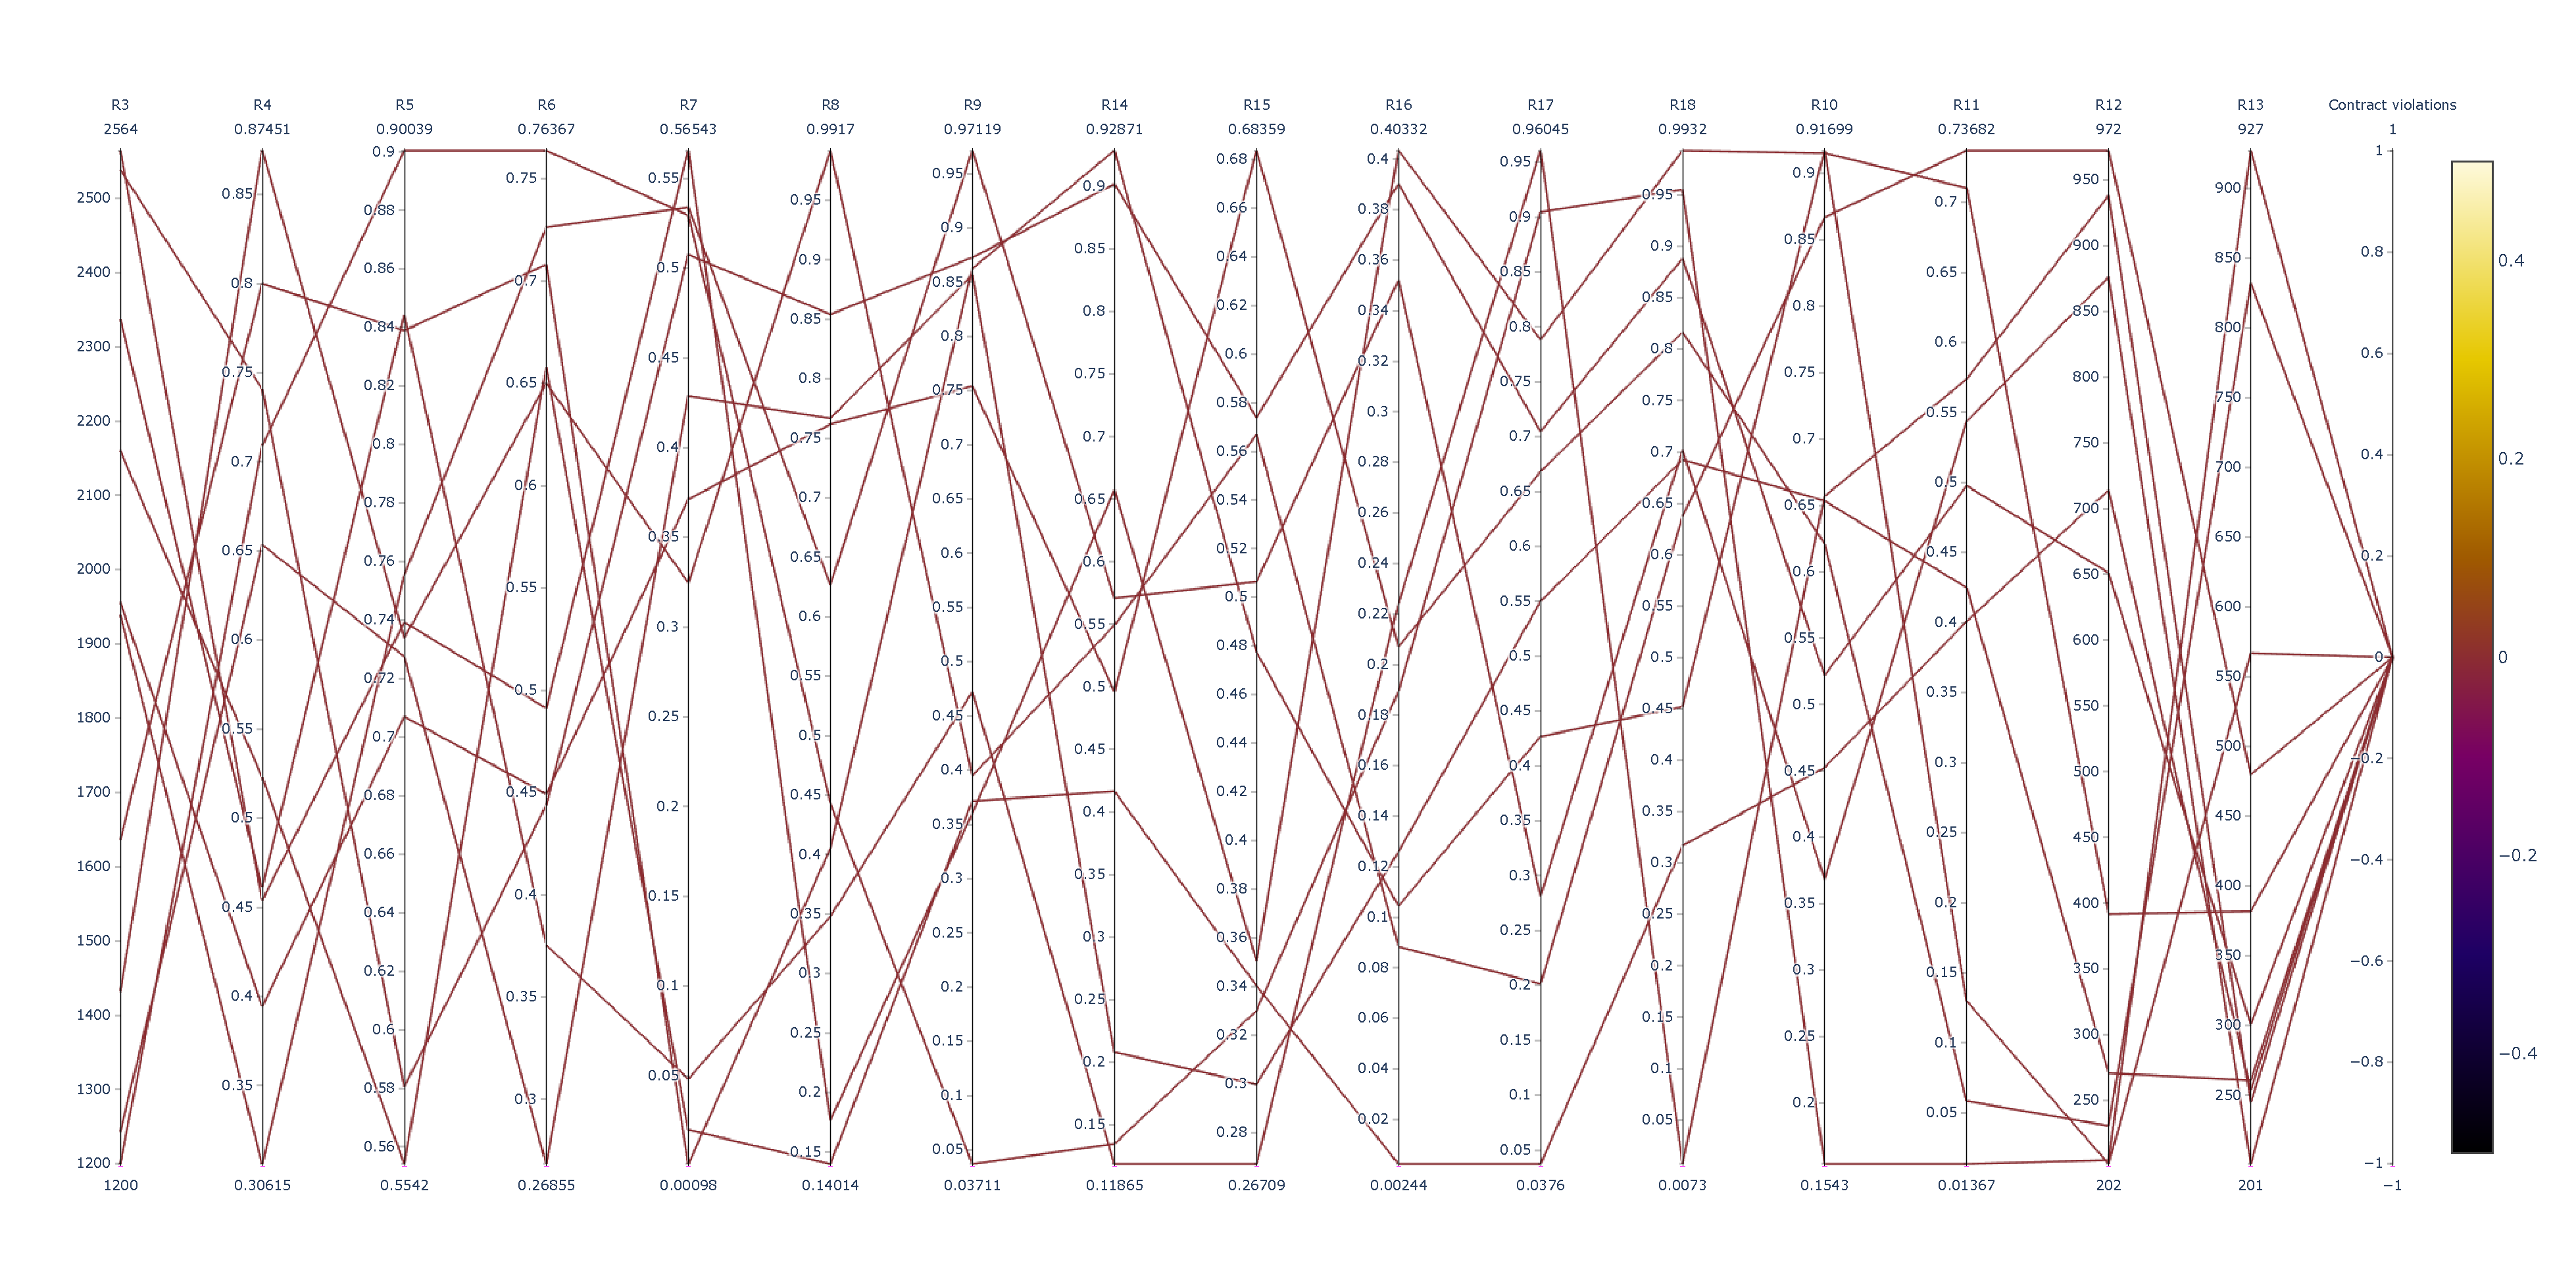
\includegraphics[width=\textwidth]{images/SPEA2_Zero_validity.html.pdf}
	\caption[]]{}
	\label{fig:SearchSpaceValid}
\end{figure}

If we are filtering out all configurations that gave not valid results, we obtained the search space a few that contain only valid results. A parallel plot that demonstrates this situation showed in Figure~\ref{fig:SearchSpaceValid}. The plot shows that many configurations give a valid result for the specified problem. However, still, there are no visible dependencies between the parameters and the number of contract violations, or between the parameters themselves.

\begin{figure}
	\centering
	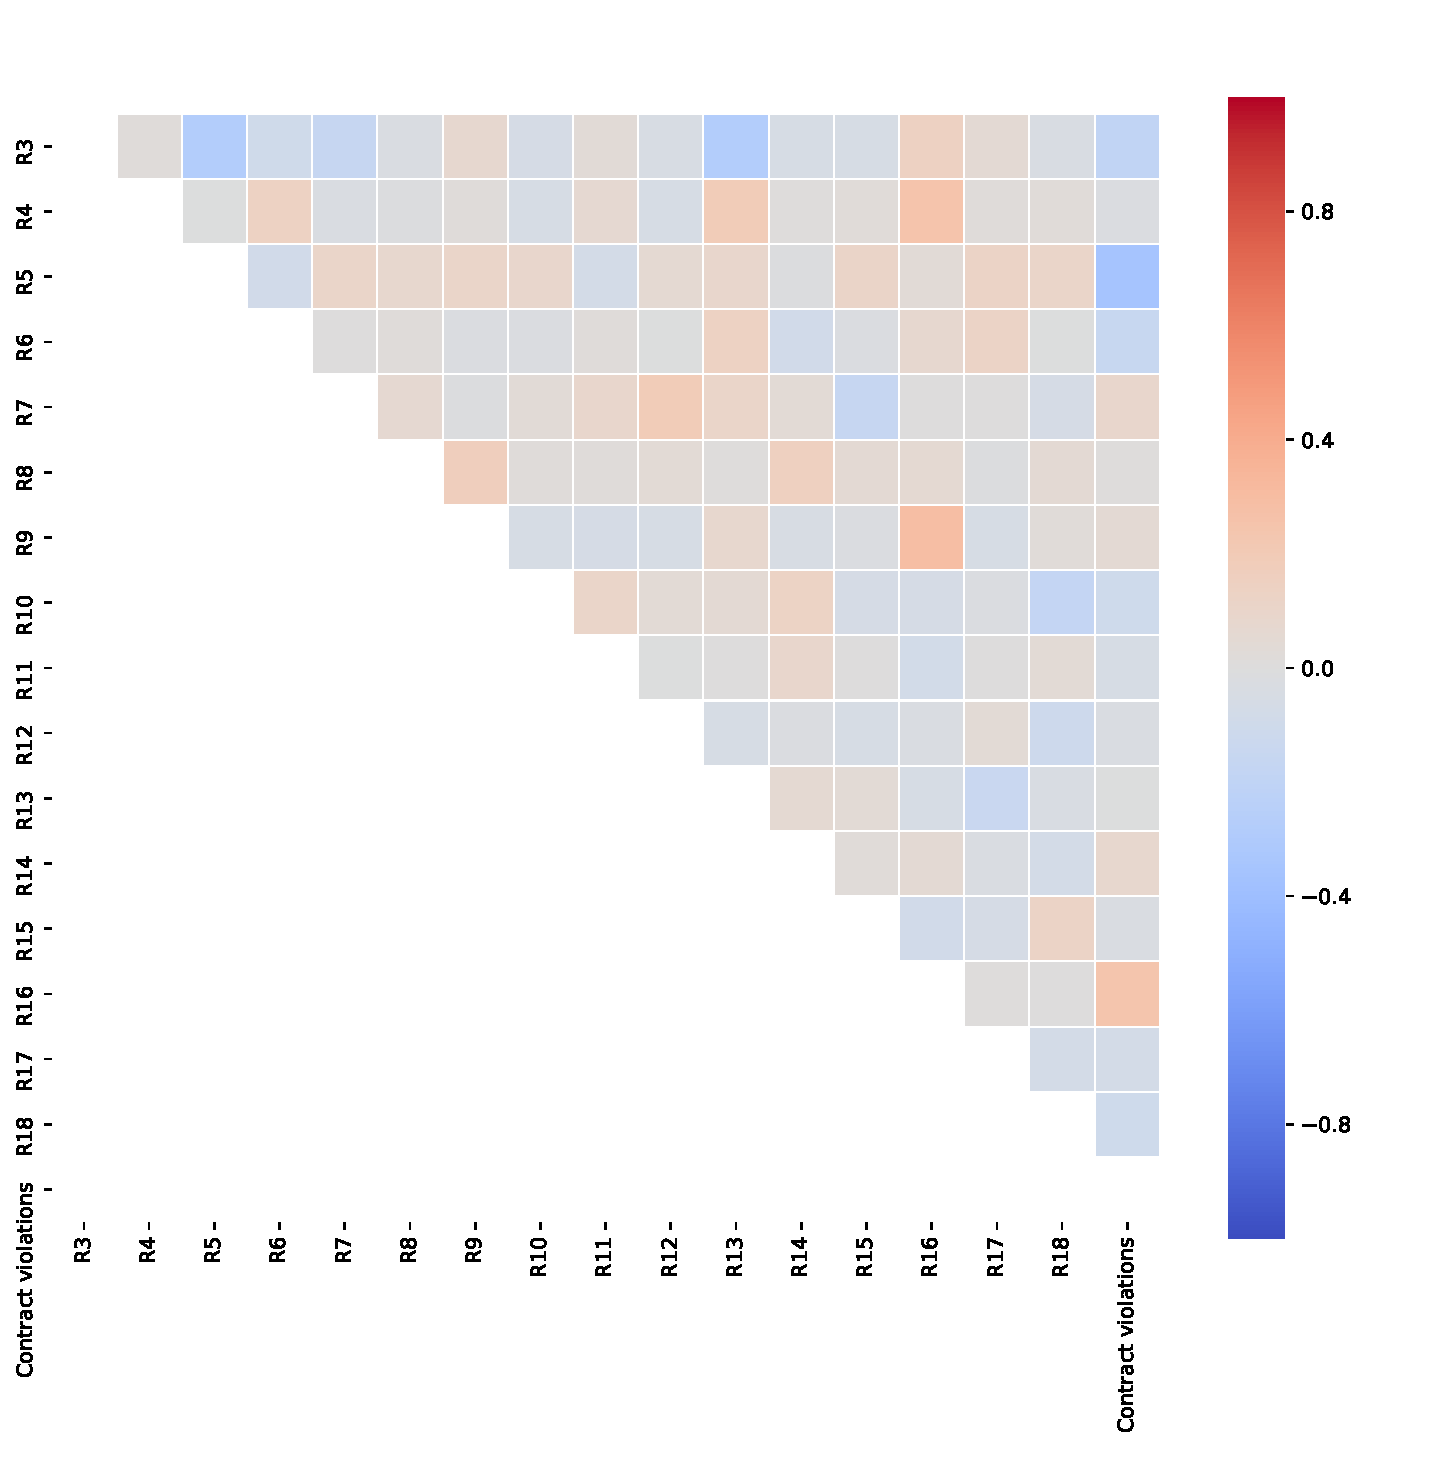
\includegraphics[width=\textwidth]{images/CorrelationAnalysis.pdf}
	\caption[]]{}
	\label{fig:CorrelationAnalysis}
\end{figure}

Cause Figure~\ref{fig:SearchSpaceViewFull} and Figure~\ref{fig:SearchSpaceValid} shows that search space view could not give any conclusions about dependencies between parameters or between parameters and number of contract violations, another method of analysis was performed.

To get information how parameters relay on each others the correlation analysis was performed and results showed in Figure~\ref{fig:CorrelationAnalysis}.

\todoR{I stopped here}


Colors indicate the level of correlation. Blue is the inverse correlation, that means that bigger value of parameter gives smaller number of contract violations. Red color means that bigger value o parameter gives bigger number of contract violations.
From the correlation analysis, we can conclude that there are no strong dependencies between the number of contract violations and parameters. There are two more important parameters: \texttt{CrossoverRate}(R5) and \texttt{CrossoverOnRandomRequestProbability}(R16).
Correlation analysis showed that the \texttt{CrossoverRate} need to has a big value. Also, conclusion from this analysis that small value  \texttt{CrossoverOnRandomRequestProbability}. It's also shows that we can remove this parameter. 

For further analysis of dependencies, graphs of the distribution of parameter pairs were constructed. Let us examine one representative distribution and, using another as an example, show how others look.

\begin{figure}
	\centering
	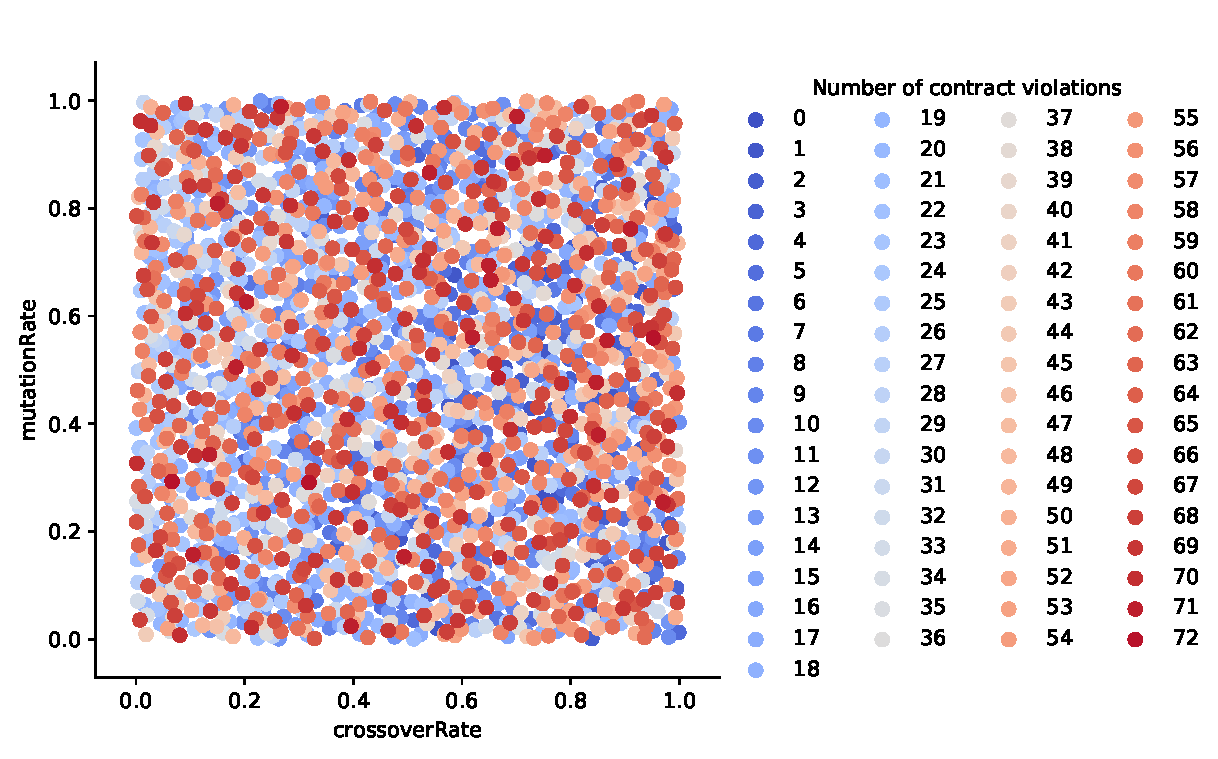
\includegraphics[width=\textwidth]{images/CrossoverRateVsutationRate.pdf}
	\caption[]]{}
	\label{fig:CrossoverRateVmutationRate}
\end{figure}

\begin{figure}
	\centering
	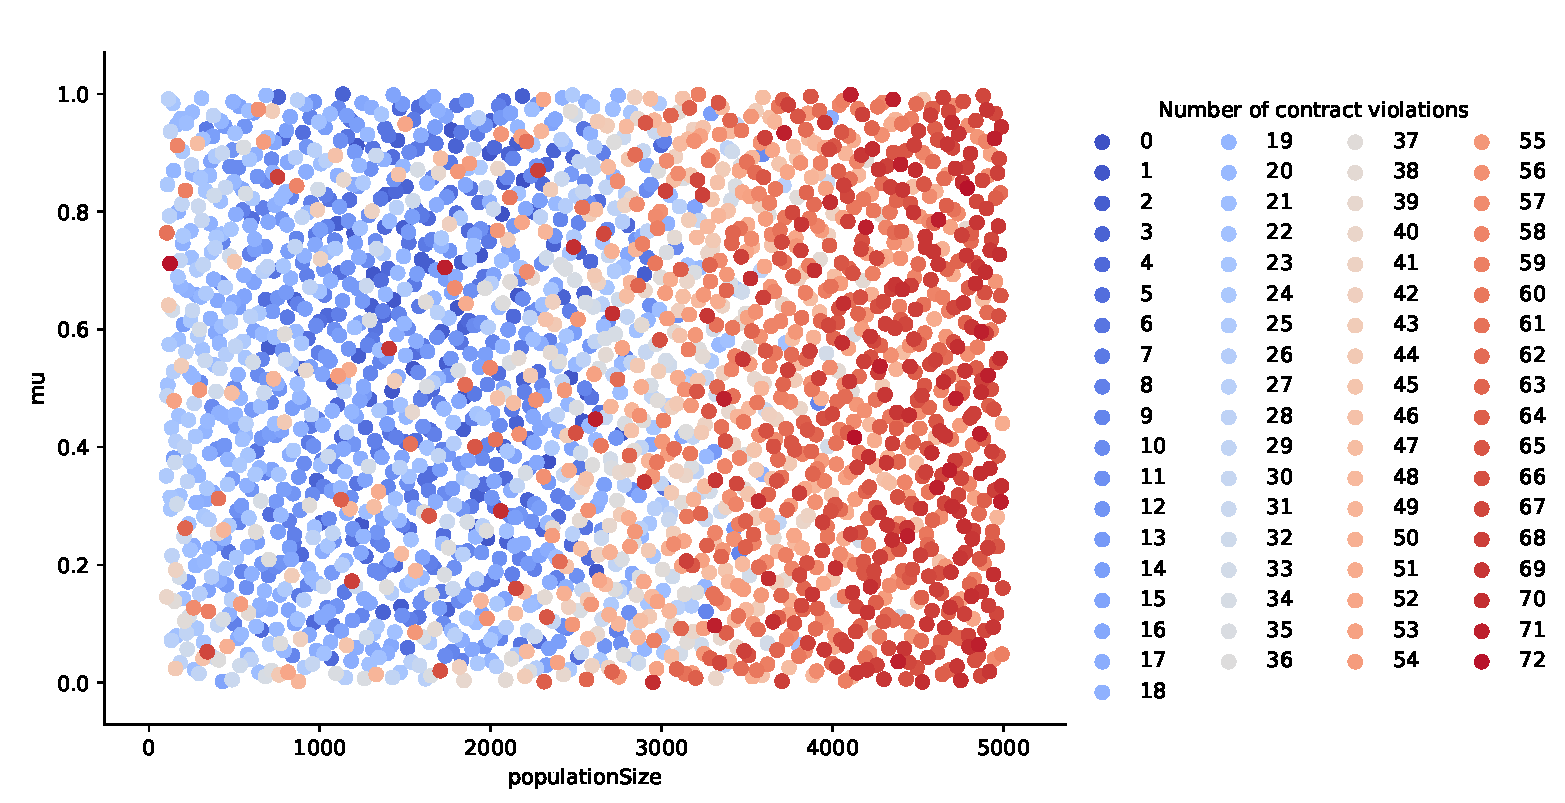
\includegraphics[width=\textwidth]{images/populatioSizeVsMu.pdf}
	\caption[]]{}
	\label{fig:populatioSizeVsMu}
\end{figure}

Any distribution associated with the population size parameter has a different look and shows that this parameter has an effect on the result.
Figure~\ref{fig:populatioSizeVsMu} shows an example of such distribution, and it is clearly seen that valid results, or close to valid, are in the range from 1000 to 2600.

At the same time, most distributions are similar to Figure~\ref{fig:CrossoverRateVsutationRate}, which shows the distribution of parameters of crossover rate and mutation rate. 
The Figure~\ref{fig:CrossoverRateVmutationRate} shows that valid, or close to valid results exist for all values of described parameters. That also confirms idea described in correlation analysis to remove some parameters like \texttt{CrossoverOnRandomRequestProbability} from the tuning and set it in the solver as 0.

\begin{figure}
	\subfloat[Name A]{%
		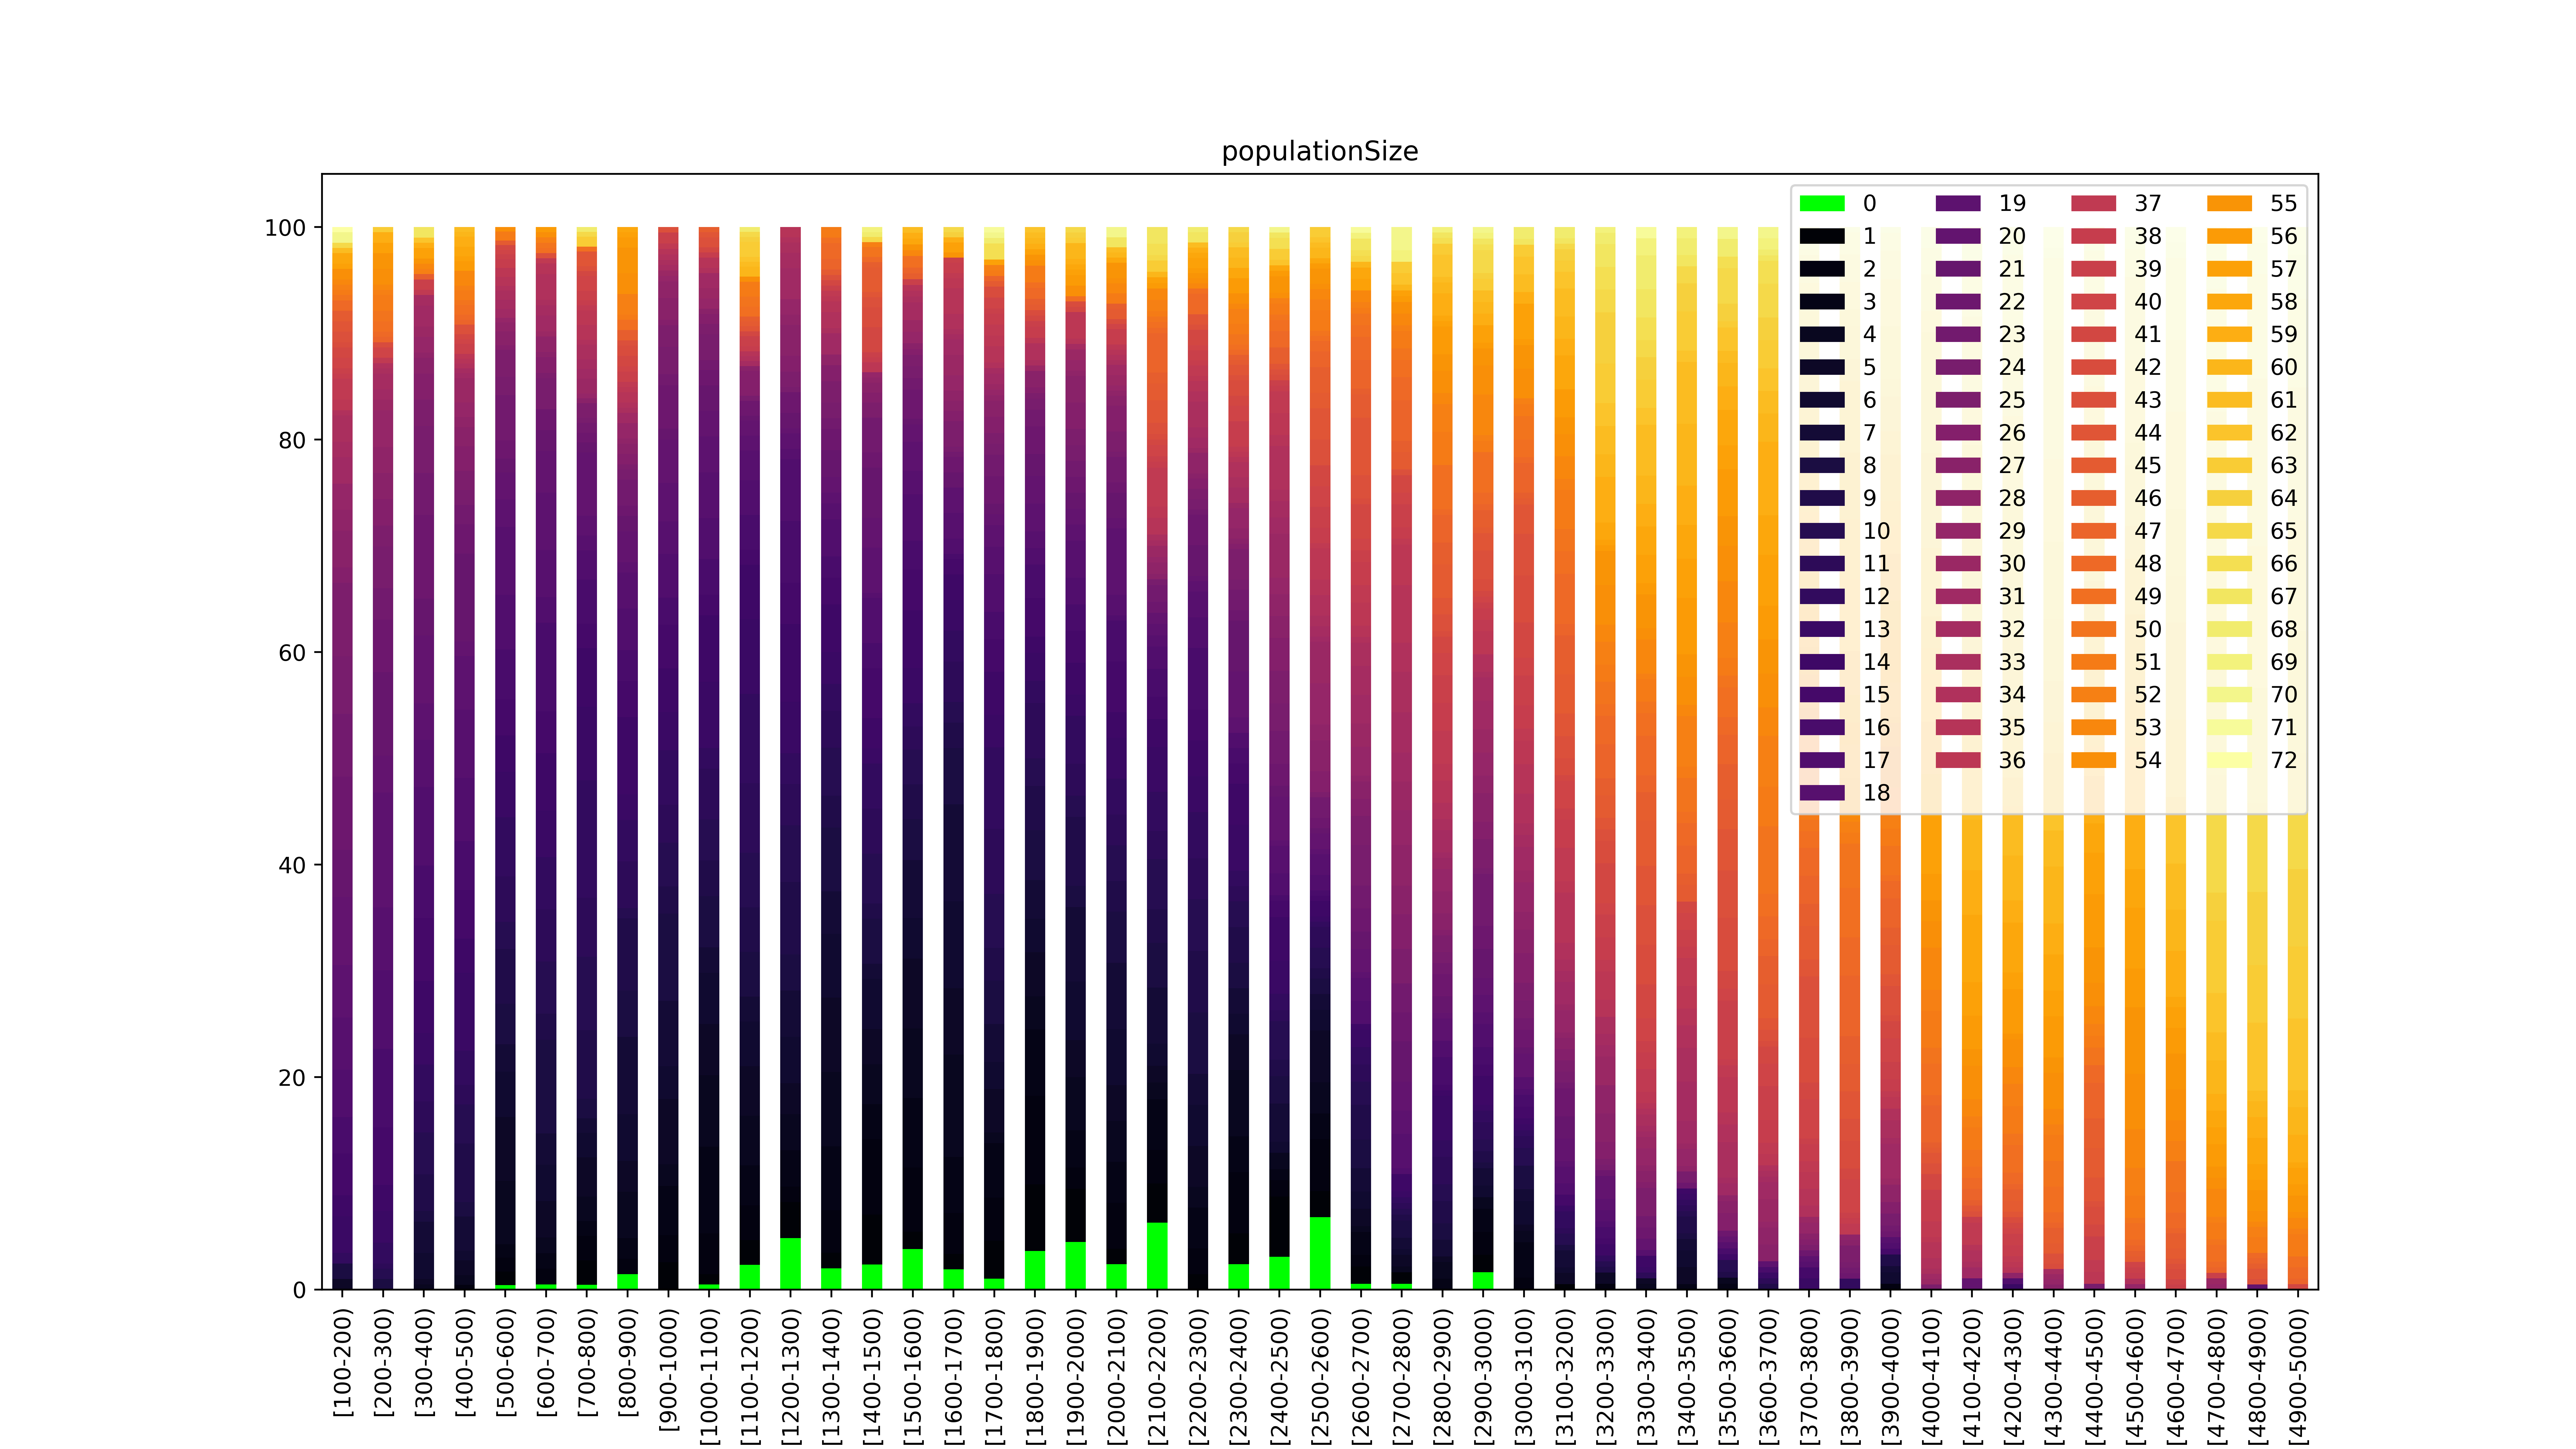
\includegraphics[clip,width=\textwidth]{images/populationSize_gradientBig.png}%
	}
	
	\subfloat[Name b]{%
		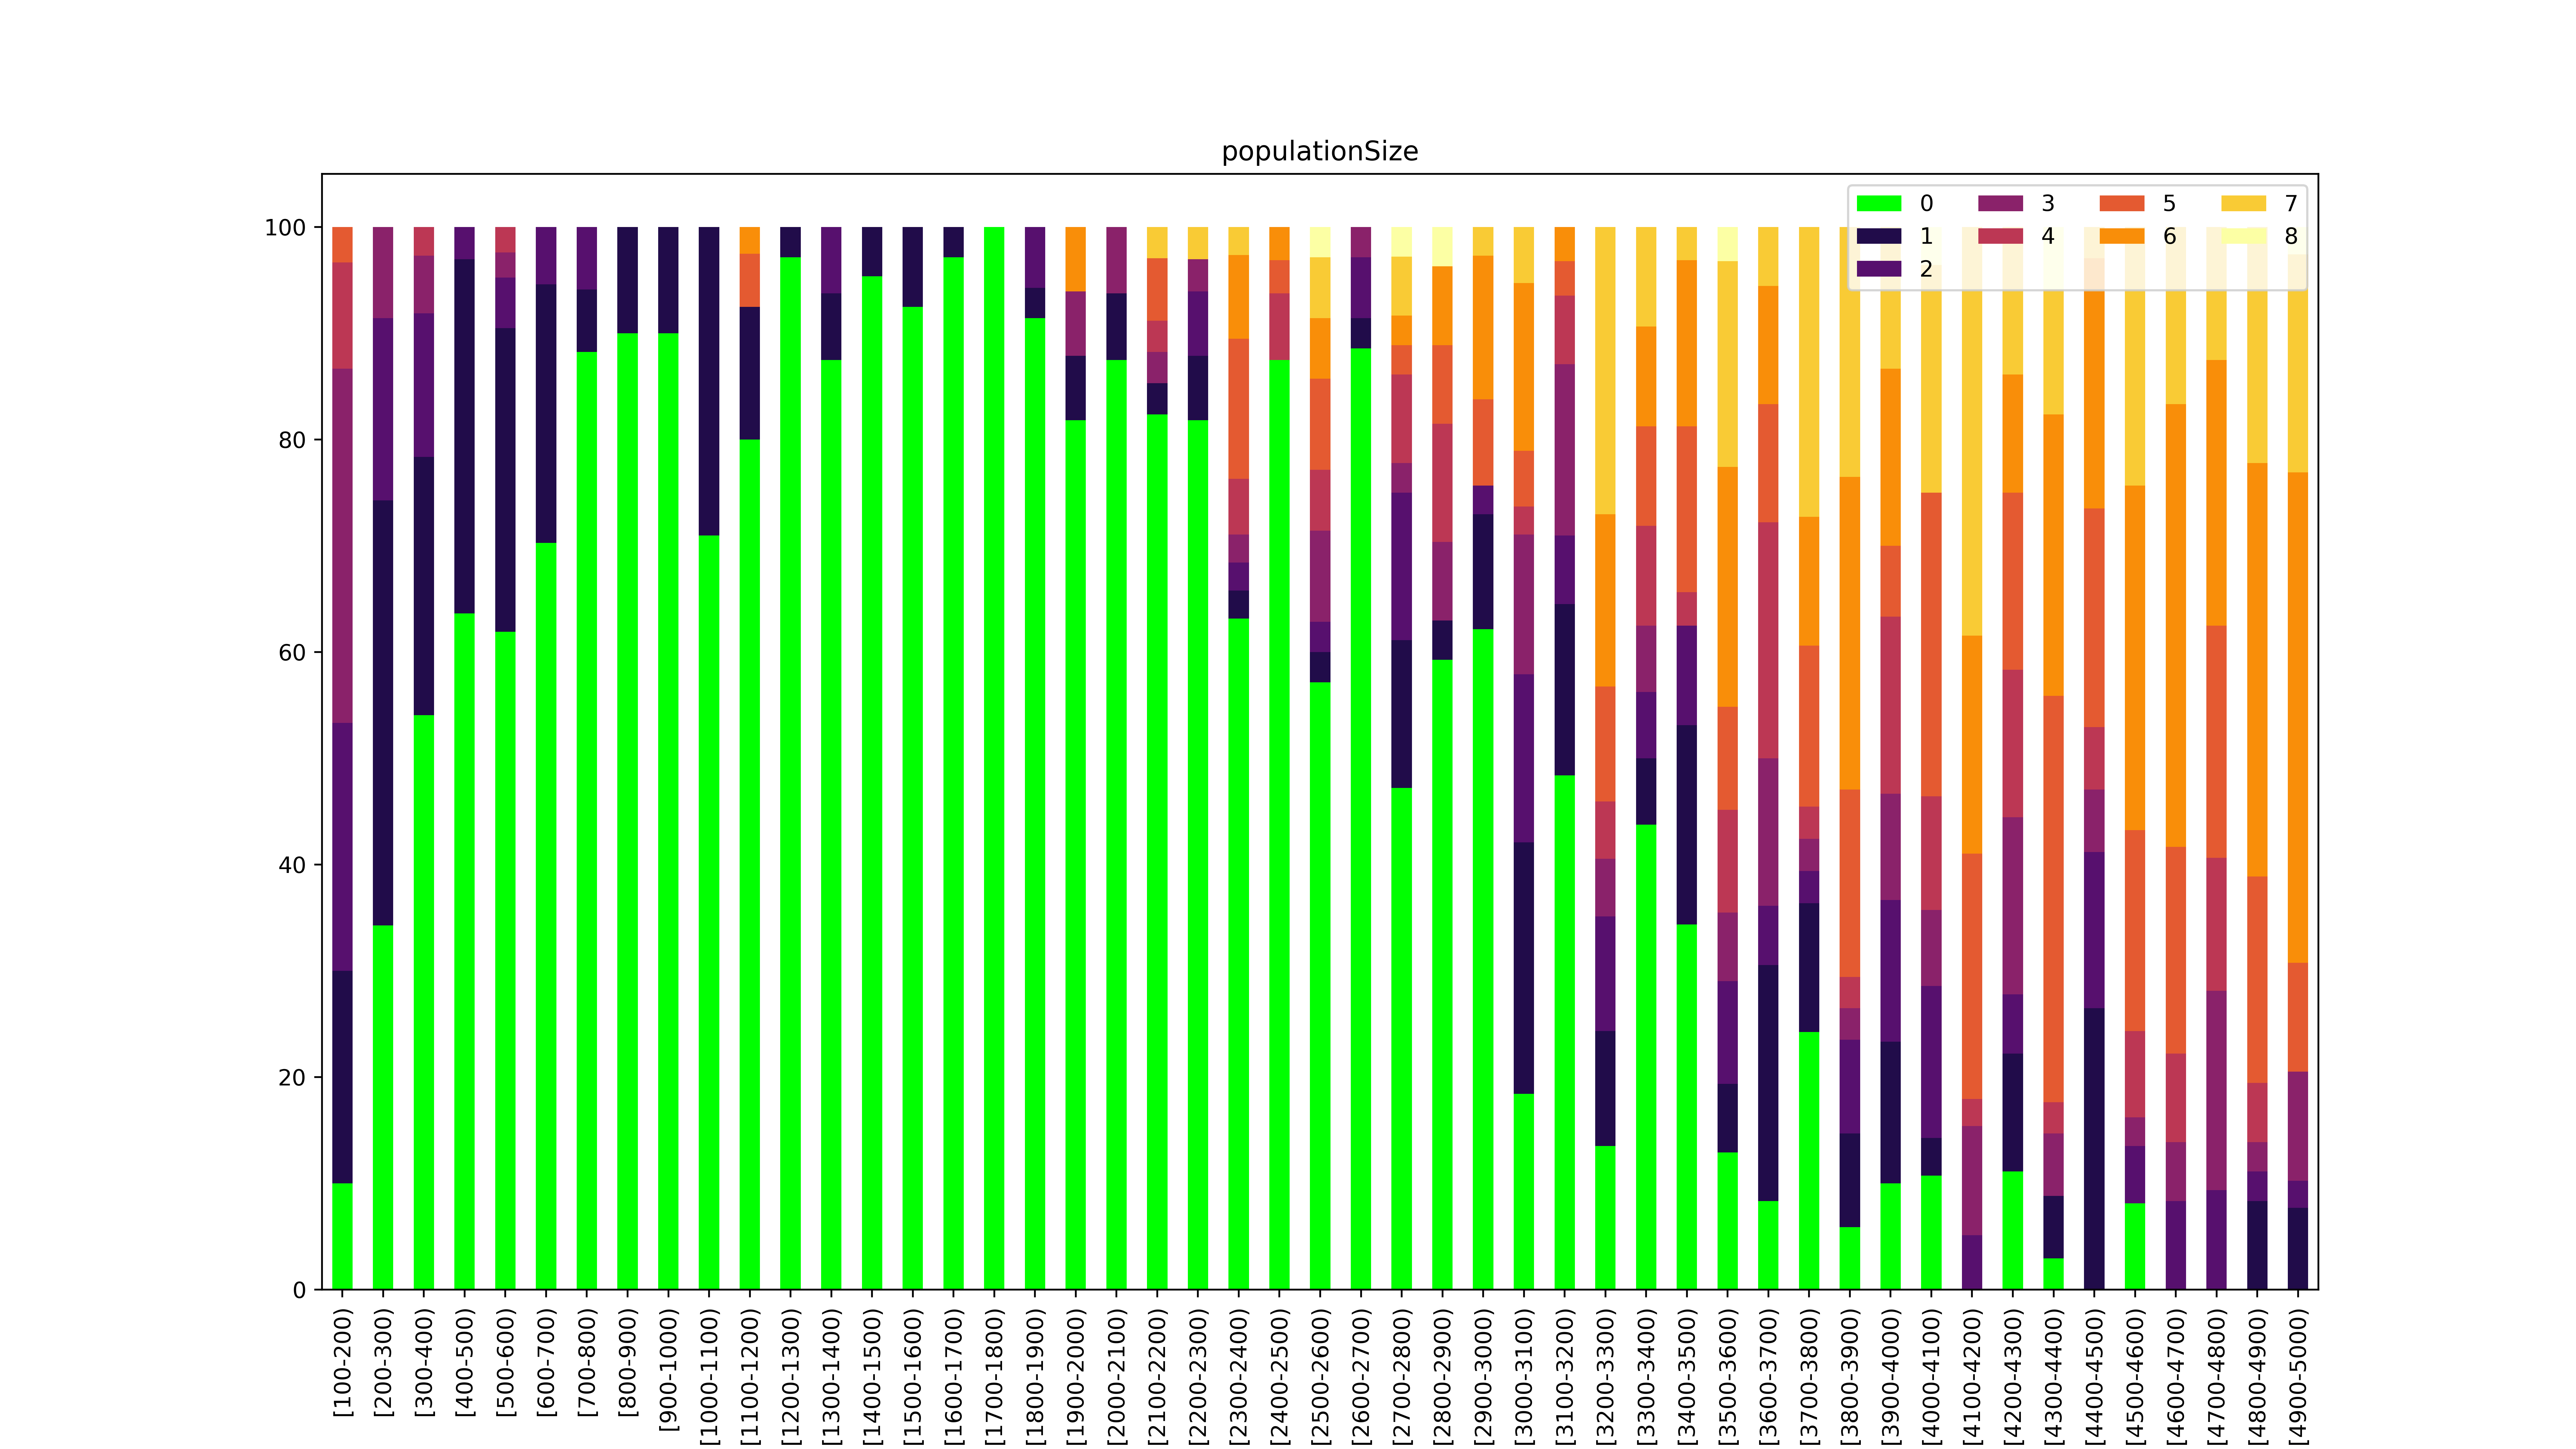
\includegraphics[clip,width=\textwidth]{images/populationSize_gradientSmall.png}%
	}
	
	\caption{main caption}	
\end{figure}

The next step in the analysis is the distribution of the parameter value and the number of contract violations that he gave. Consider the distribution of the population size parameter.
The color indicates the number of contract violations. The column height of a specific color is a percentage of the total number of configurations that have the same value. As can be seen, valid solutions are in the range from 1000 to 2600, which confirms the conclusion from the last step.

For a more visual image, we construct a similar graph for the smaller problem. This problem described with parameters: variants - 2, depth - 2, requests - 2, resources - 5.
It is shown in Figure~\ref{fig:populationSize_gradientSmall}. If we compare Figure~\ref{fig:populationSize_gradientSmall} and Figure~\ref{fig:populationSize_gradientBig}, we can see that they have a similar distribution.

\begin{figure}
	\centering
	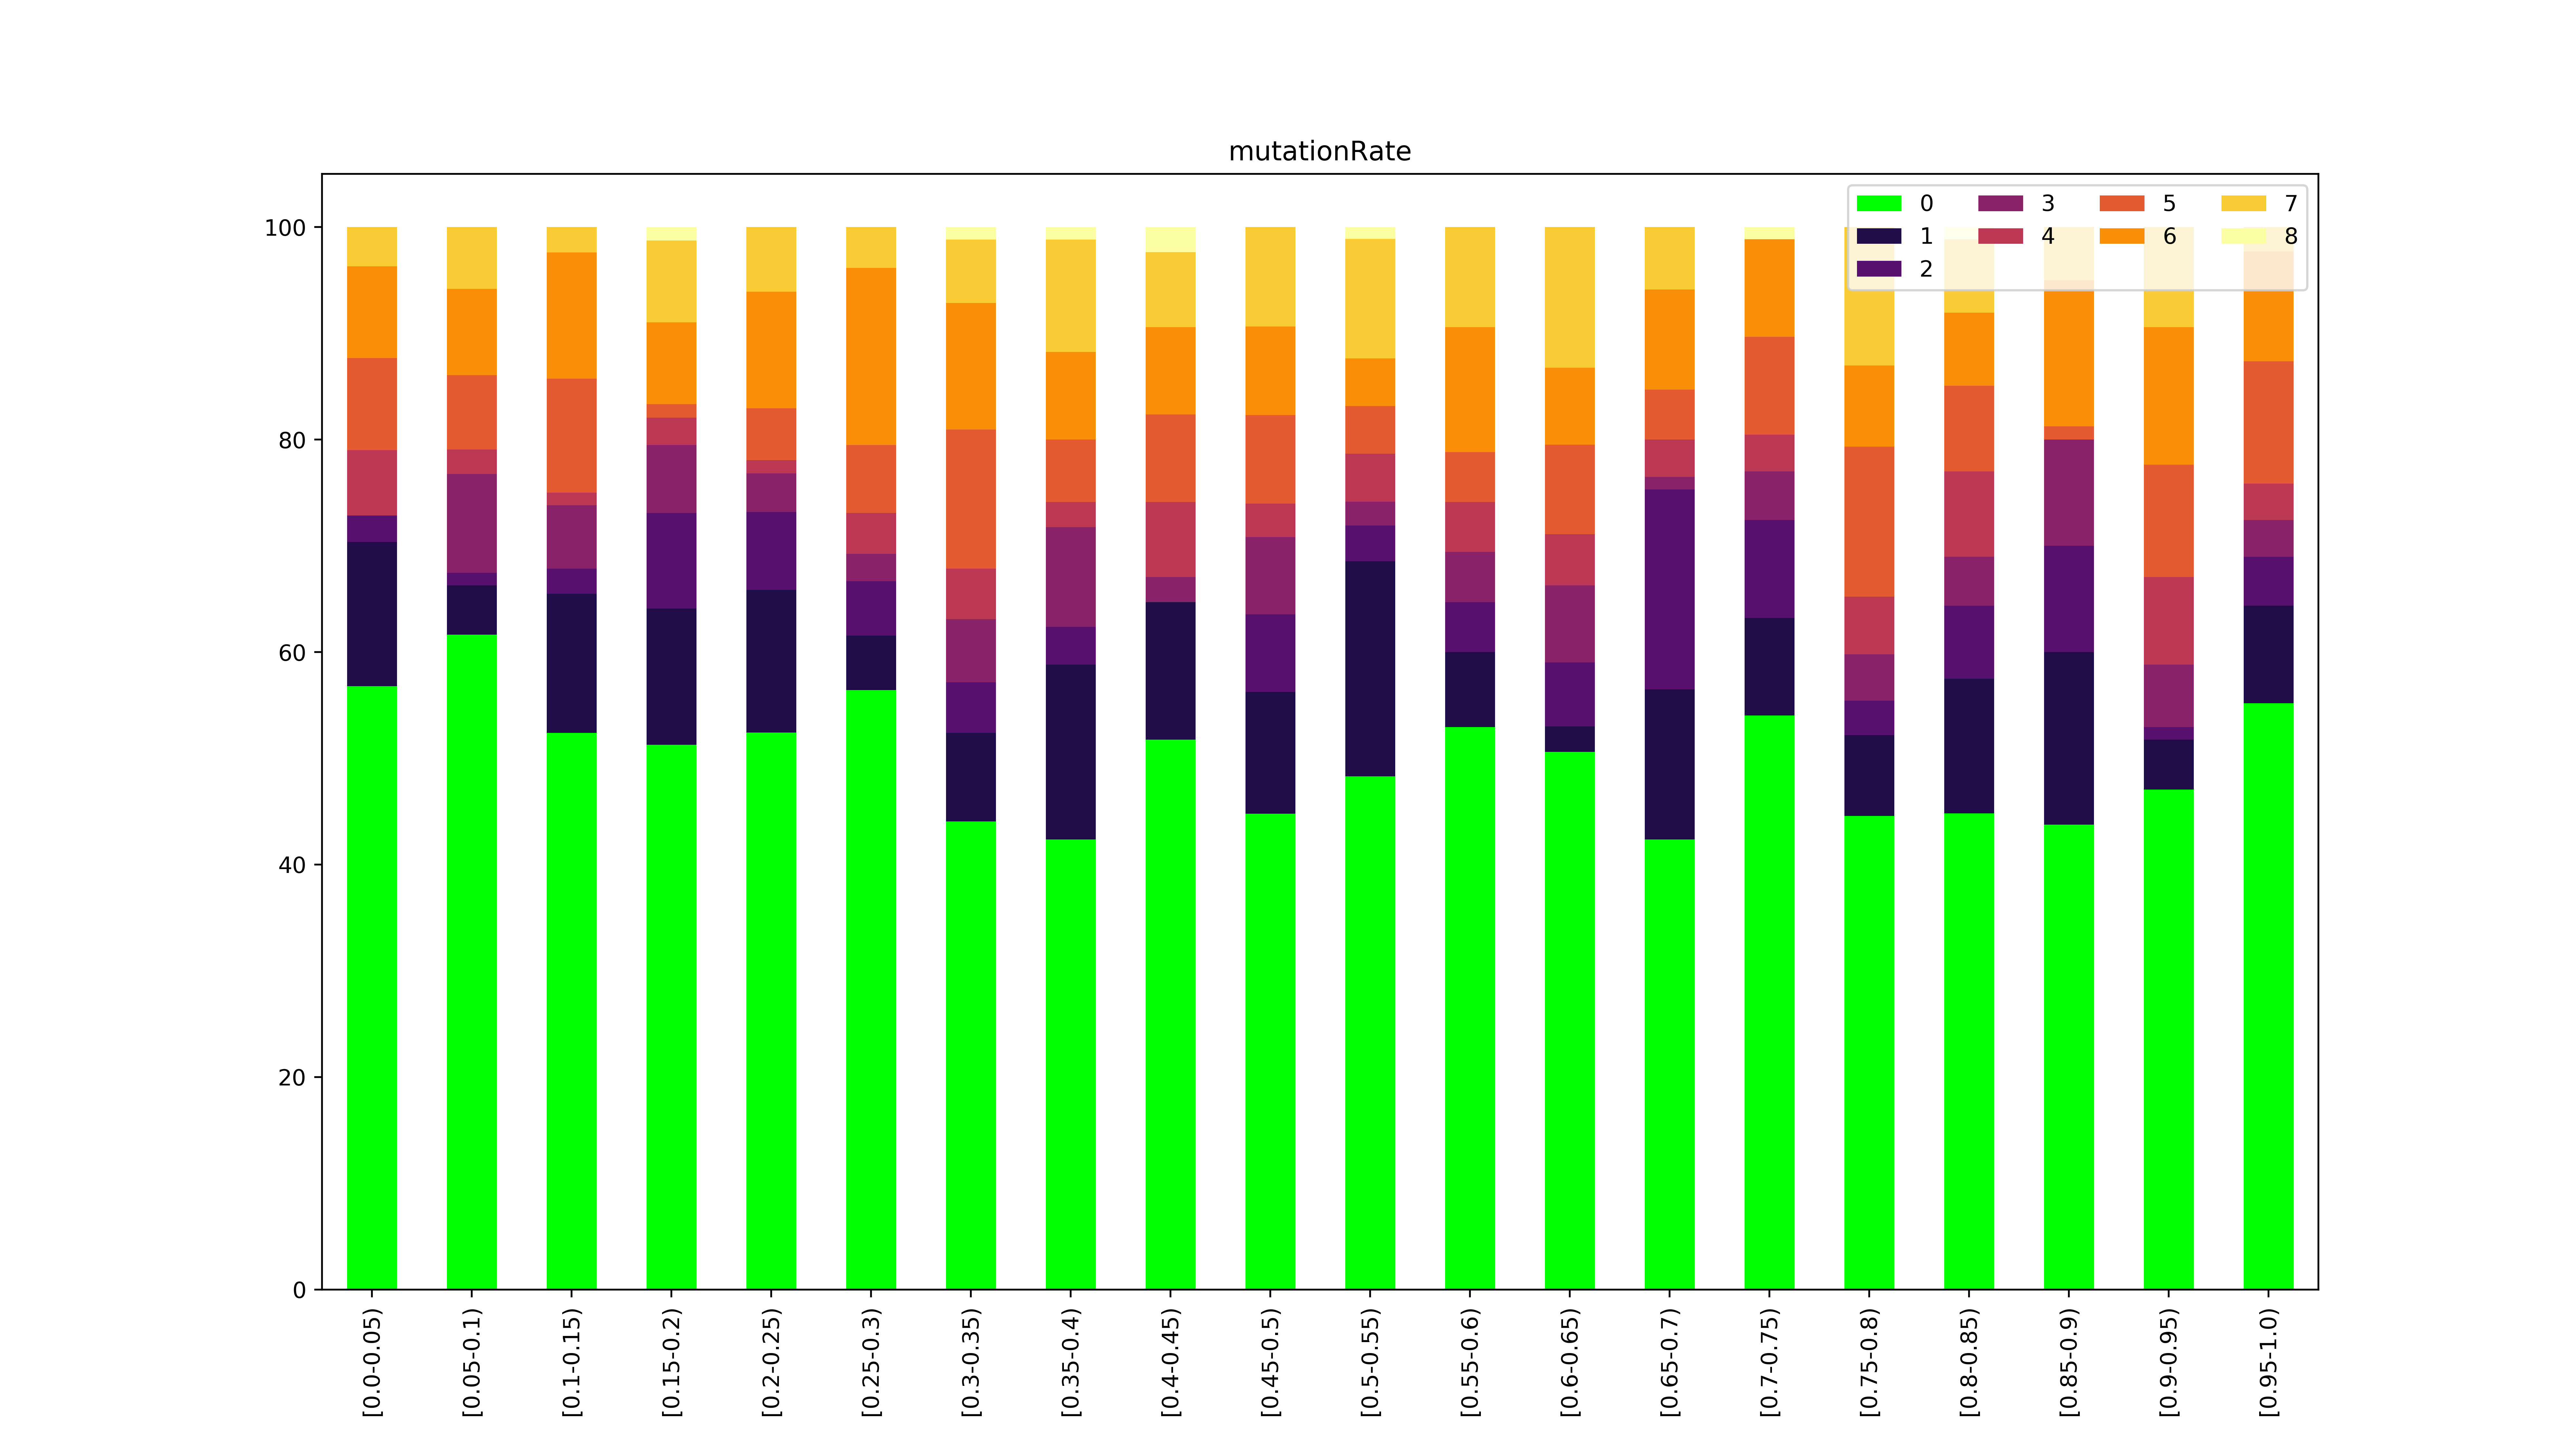
\includegraphics[width=\textwidth]{images/mutationRate_gradient_500dpi.png}
	\caption[]]{}
	\label{fig:mutationRate_gradient}
\end{figure}

The distributions of most parameters look like the distribution of the mutation rate parameter outlined in Figure~\ref{fig:mutationRate_gradient}.

Such a distribution means that the result of the solver does not matter from the value of the specific parameter.

\begin{figure}
	\centering
	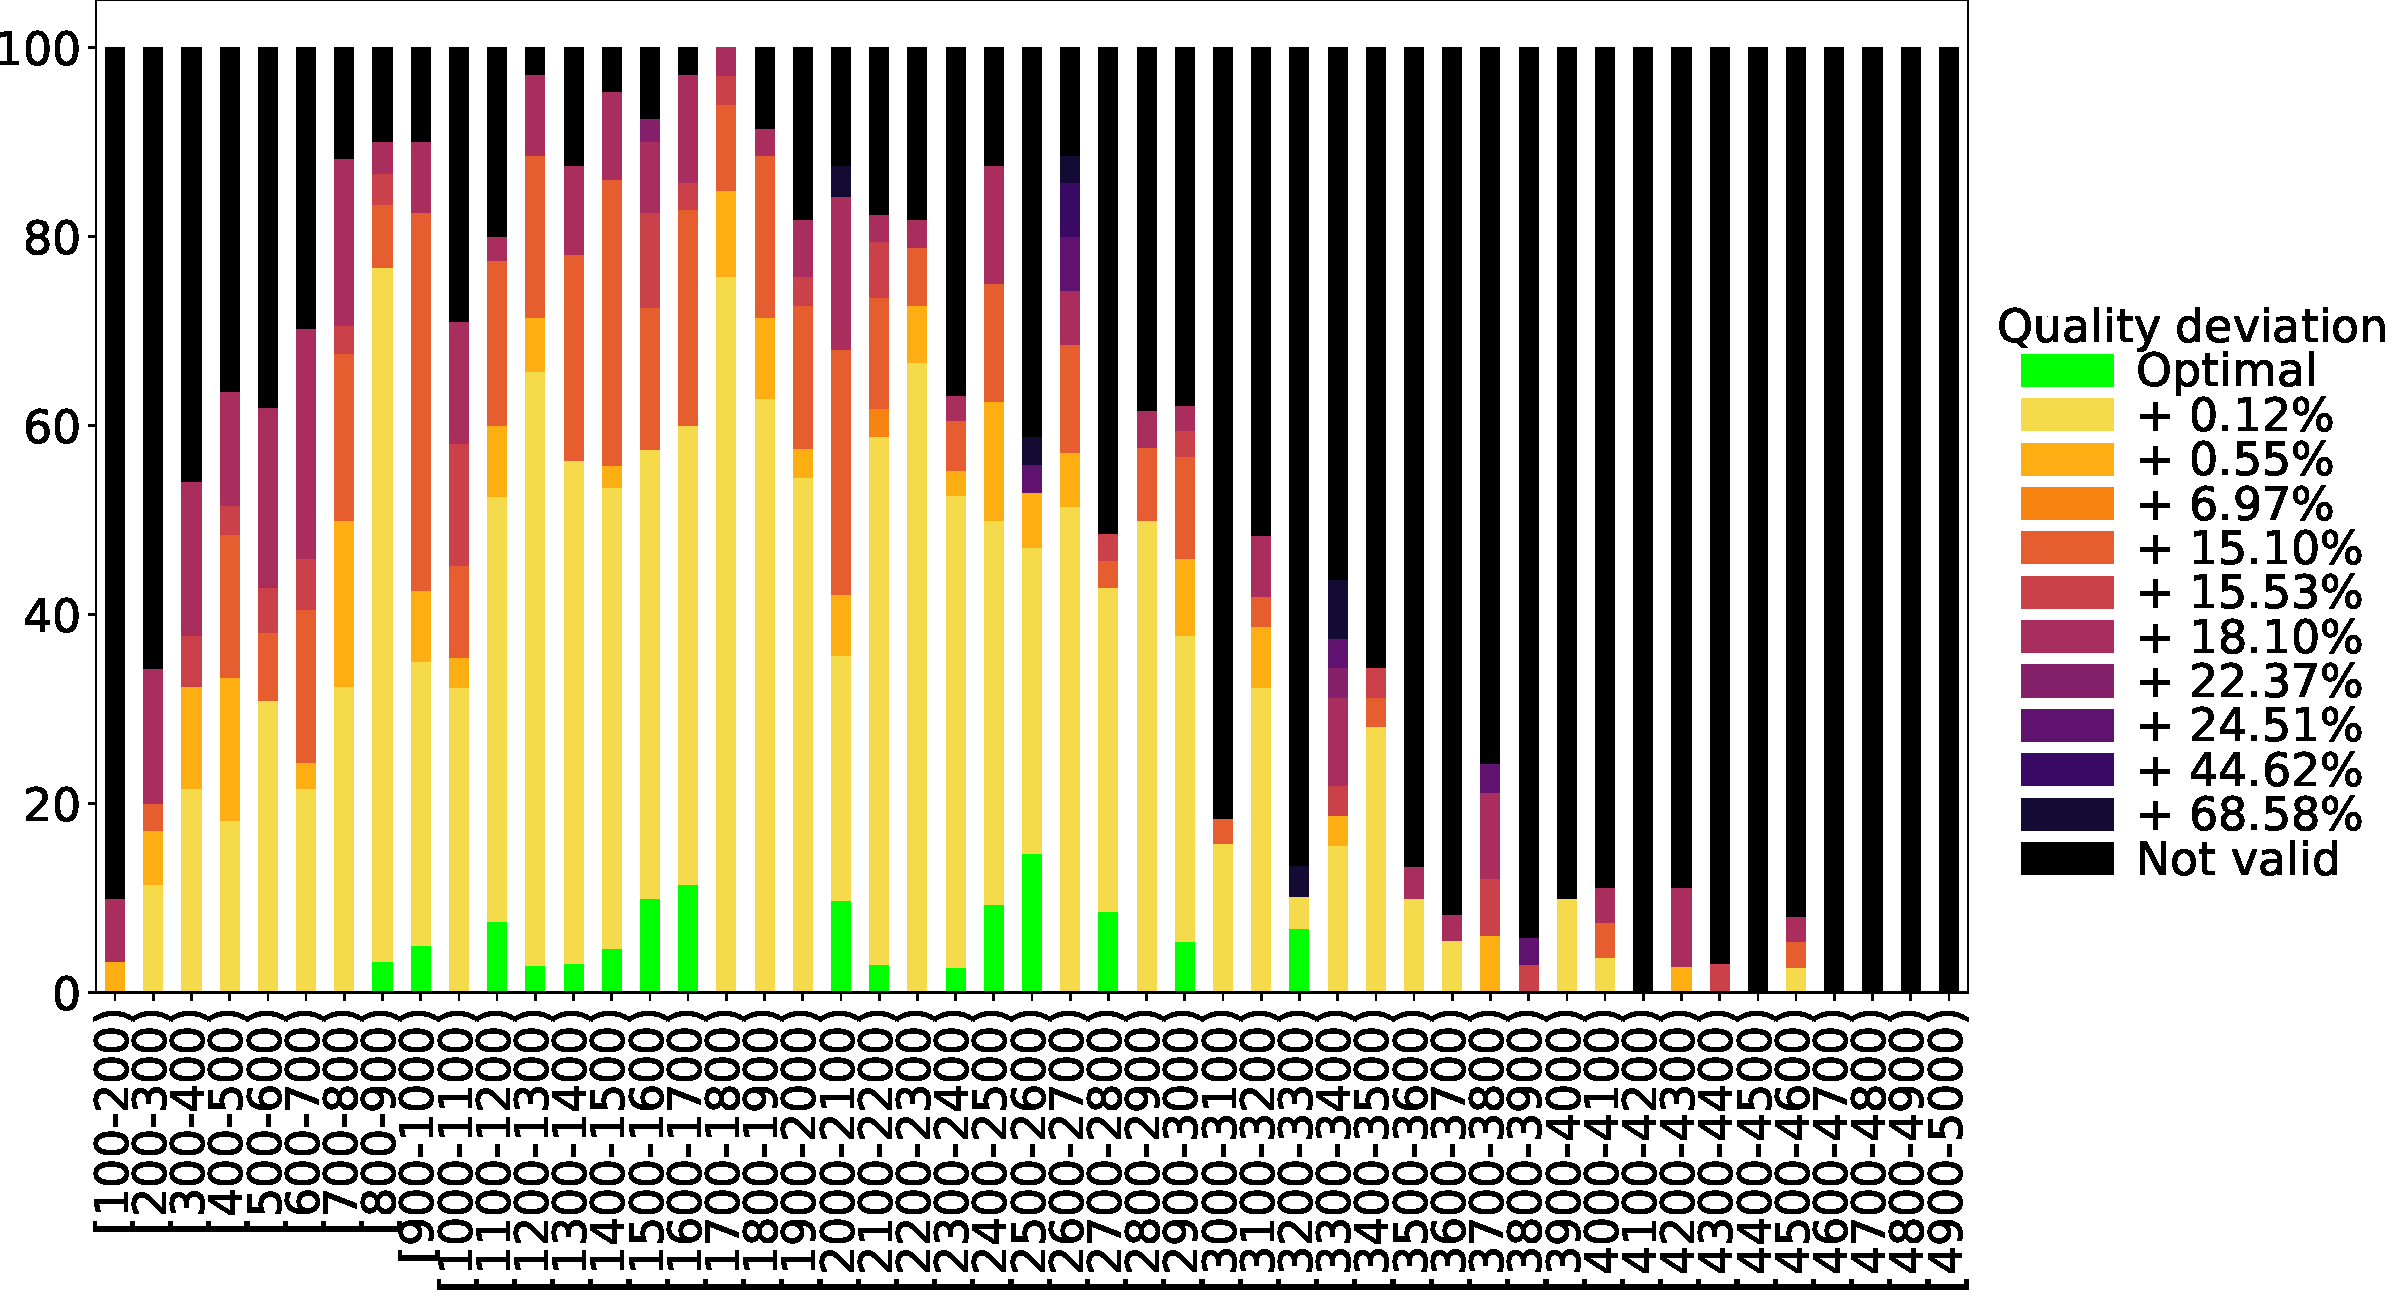
\includegraphics[width=\textwidth]{images/populationSizeObjective.pdf}
	\caption[]]{}
	\label{fig:populationSizeObjective}
\end{figure}

As for energy, let's build the distribution of the obtained energy values for the same parameters (Figure~\ref{fig:populationSizeObjective}).

This distribution proves the fact that if the solver found a valid solution, then this solution is optimal, or close to it.